\documentclass[withoutpreface,bwprint]{cumcmthesis} %去掉封面与编号页，电子版提交的时候使用。


\usepackage[framemethod=TikZ]{mdframed}
\usepackage{url}   % 网页链接
\usepackage{subcaption} % 子标题
\usepackage{listings}  % 导入listings包
\usepackage{xcolor}    % 支持颜色设置
\title{基于遗传算法的无人机投弹策略优化}
\tihao{A}
\baominghao{4321}
\schoolname{XX大学}
\membera{ }
\memberb{ }
\memberc{ }
\supervisor{ }%辅导老师
\yearinput{2025}
\monthinput{9}
\dayinput{7}

\begin{document}

\maketitle

\begin{abstract}

	为应对来袭导弹对固定圆柱体目标的打击，本文围绕“无人机投放球状烟雾”的软杀伤方案，提出一套基于\textbf{遗传算法}并辅以\textbf{贪心算法}优化，采用从几何评估到协同优化的一体化方法。本文构建了导弹匀速，无人机等高匀速直线运动，干扰弹平抛运动，球状烟雾下沉的运动学模型。并且构建了基于圆柱体目标表面采样的\textbf{“严格全覆盖”}判据，形成通用评估内核；在此基础上，还结合遗传算法的“粗筛+细筛”，使用贪心算法分解问题，采用上界剪枝与结果缓存等工程化策略，进行系统求解。
	
	\textbf{问题一：}  统一构建“导弹——无人机——干扰弹”运动学模型，给出导弹所在点到圆柱体上每一点实现均被烟雾球遮挡的严格遮蔽判据；在统一时间窗内返回遮蔽区间并计时，得到单弹确定参数的情况下的遮蔽时间为\textbf{1.39s}，由此确定后续各题共用的评估内核与输出格式。
	
	\textbf{问题二：}  采用遗传算法 \textbf{全局搜索}，粗评用较大步长与快速充分判据预筛，精评以小步长按严格口径重估，并通过可行化修复满足起爆时限与最短间隔，找到最优的航向，速度，投放时刻与起爆延迟，得到单机单弹最长遮蔽时间为\textbf{4.58s}。

	\textbf{问题三：}  在问题二的框架内优化三次投放时序与延迟，以遮蔽区间并集计分（重叠不重复计时）；编码采用差分间隔以保证最短投放间隔，评估仍调用问题1的严格判据。得到最长遮蔽时间为\textbf{6.40s}，验证“拼窗延时”策略的有效性与稳健性。

	\textbf{问题四：}  本题将问题扩展至三架无人机，因此本文先以贪心策略分别求出三机单机最优并筛为高价值种子，再注入遗传算法做协同细化；总体指标为三机遮蔽区间的并集长度。最终得到三机并集遮蔽时间为\textbf{11.38s}。

	\textbf{问题五：}  本题扩展五机三干扰弹三导弹，极大增加了复杂度，本文采用贪心策略将问题分解，对每枚导弹分别计算各机三弹的并集时长，再对三枚导弹求和作为每机得分，最后汇总五机总分；为加速评估与迭代，引入上界剪枝与结果缓存并保留严格口径终评。最终获得总有效遮蔽 \textbf{22.27s}。

\keywords{优化问题\quad	  遗传算法\quad  智能优化算法\quad   贪心算法\quad}

\end{abstract}

\section{问题重述}

\subsection{问题背景}

现代战争中，精确制导武器对高价值固定目标的打击能力日益增强，传统硬杀伤拦截手段面临成本高、响应慢、拦截窗口短等现实瓶颈。烟幕干扰作为一种典型的软杀伤防护手段，通过在短时间内形成高浓度气溶胶云团，对敌方光学、红外、激光等制导系统实施遮蔽与误导，具有成本低、部署快、效费比高等显著优势，已成为要地防空、目标防护的重要补充手段。

近年来，随着无人机技术的迅猛发展，利用具有长续航能力的无人机挂载烟幕干扰弹实施前置式、精准式干扰成为研究热点。相较于传统地面固定发射或有人机临空抛撒，无人机具备任务灵活性强、部署空域广、响应速度快等优势，可在导弹来袭航路前方预设干扰走廊，实现"以逸待劳"式遮蔽，显著延长有效干扰时间窗口。

然而，无人机烟幕干扰弹的实战效能受多重因素耦合影响：一方面，导弹飞行速度快、航路预测误差小，要求干扰云团必须在时空维度上精准遮蔽其制导视野；另一方面，烟幕云团以恒定速度下沉、有效遮蔽半径有限、持续时间短暂，需通过多弹协同、起爆时序优化、航路动态规划等手段，实现对真目标的有效遮蔽时长的最大化。此外，无人机在受领任务后可瞬时调整航向与速度，但一旦确定即不再变更，这使得投放点、起爆点、航路参数必须在任务初始阶段一体化优化，构成了典型的多约束、多阶段、多目标决策问题。

在此背景下，如何利用有限的无人机与干扰弹资源，针对多枚来袭导弹，设计时空协同的投放策略，使烟幕云团在真目标周围形成持续、稳定、高效的遮蔽屏障，成为提升要地生存概率的核心科学问题。本研究围绕该问题，构建 \textbf{多弹协同遮蔽} 模型，融合遗传算法与贪心策略，系统优化无人机飞行参数、干扰弹投放时序与起爆位置，为无人机软杀伤作战提供量化决策支持与工程可实现方案。

\begin{figure}[!h]
    \centering
    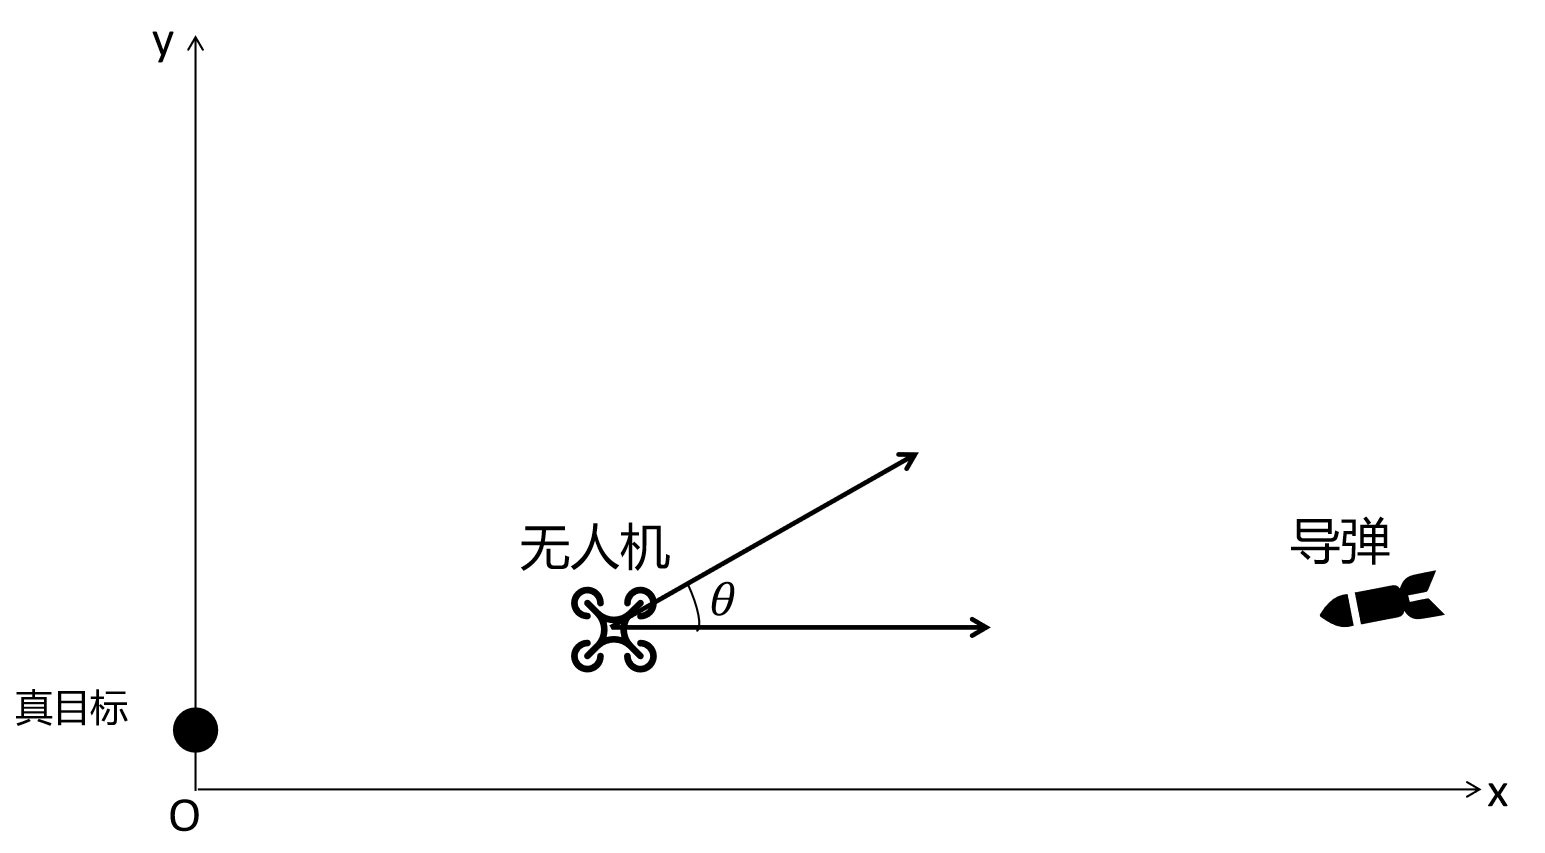
\includegraphics[width=\textwidth]{./figures/scene_overview}
    \caption{航向角说明}
    \label{fig:scene_overview}
\end{figure}

\subsection{问题提出}

\textbf{问题1：} 在无人机FY1飞行速度、飞行方向、烟幕干扰弹投放点和烟幕干扰弹起爆点均固定的情况下，如何计算烟幕干扰弹所形成的球形烟幕云团对导弹进行遮蔽的有效遮蔽时间。

\textbf{问题2：} 在无人机FY1的飞行速度、飞行方向、烟幕干扰弹投放点和烟幕干扰弹起爆点均为自变量的情况下，如何合理选择飞行速度、飞行方向、烟幕干扰弹投放点和烟幕干扰弹起爆点的数值，使得遮蔽时间最长。

\textbf{问题3：} 在无人机FY1的飞行速度、飞行方向、三颗烟幕干扰弹分别的投放点和烟幕干扰弹起爆点均为自变量的情况下，如何合理选择飞行速度、飞行方向、三颗烟幕干扰弹分别的投放点和烟幕干扰弹起爆点的数值，使得三颗烟幕干扰弹的遮蔽时间的并集最大。并且有限制条件：每架无人机投放两枚烟幕干扰弹至少间隔 1 s。

\textbf{问题4：} 在无人机FY1、FY2、FY3的飞行速度、飞行方向、各自的烟幕干扰弹投放点和烟幕干扰弹起爆点均为自变量的情况下，如何合理选择飞行速度、飞行方向、各自的烟幕干扰弹投放点和烟幕干扰弹起爆点的数值，使得三颗烟幕干扰弹的遮蔽时间的并集最大。由于本题是三架无人机各自只携带一枚烟幕干扰弹，故没有投弹时间间隔的限制，且这三架无人机有各自的飞行轨迹，故对于投弹的位置选择更为灵活。

\textbf{问题5：} 利用 5 架无人机，他们的飞行速度、飞行方向、各自的三枚烟幕干扰弹投放点和烟幕干扰弹起爆点均为自变量，如何合理选择飞行速度、飞行方向、各自的三枚烟幕干扰弹投放点和烟幕干扰弹起爆点的数值，使得对于M1、M2、M3三枚导弹的有效遮蔽时间最长。由于有三枚导弹，故有效遮蔽要求对这三枚导弹都要进行遮蔽。

\begin{figure}[!h]
    \centering
    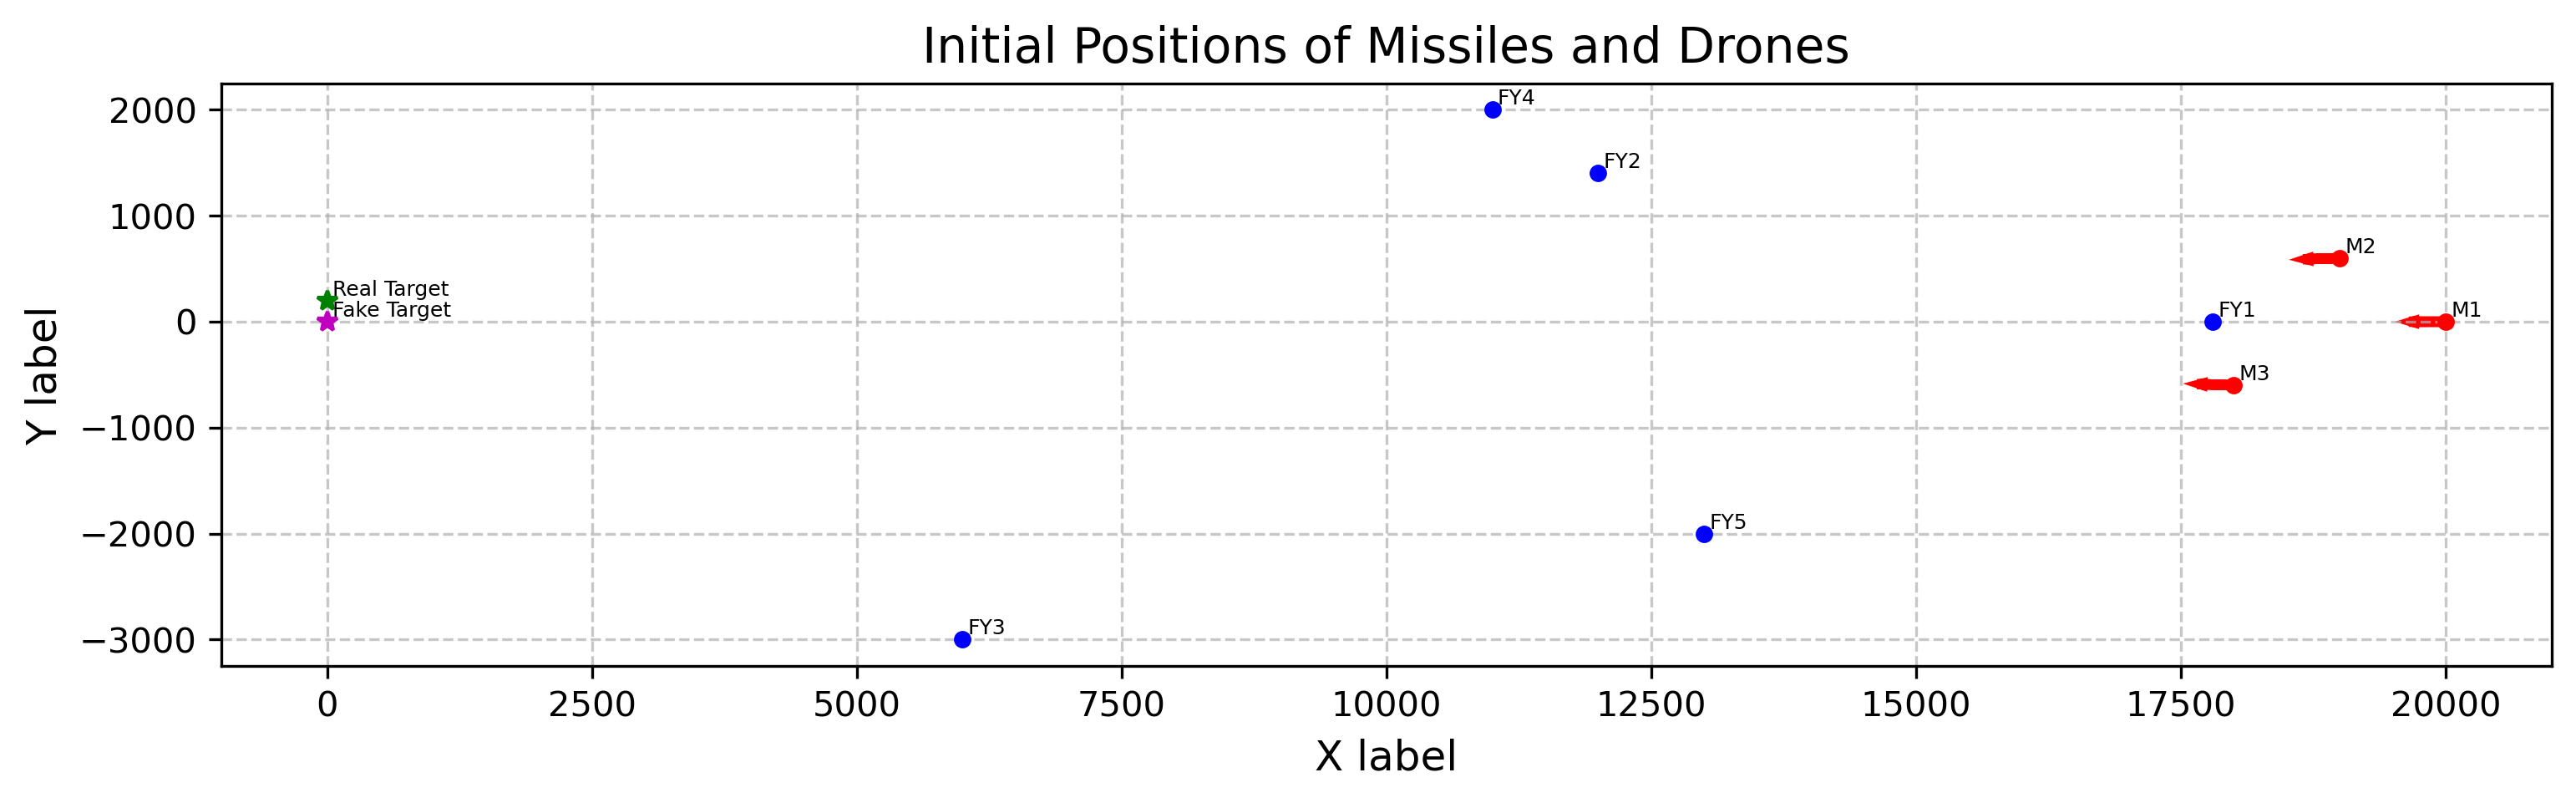
\includegraphics[width=\textwidth]{./figures/init_pos}
    \caption{无人机和导弹初始位置示意图}
    \label{fig:init_pos}
\end{figure}

\section{问题分析}

\subsection{问题一分析}

问题1要求在给定无人机FY1飞行速度、飞行方向、烟幕干扰弹投放点和烟幕干扰弹起爆点的条件下，计算单枚烟幕干扰弹对导弹M1的有效遮蔽时间。核心思路是建立导弹匀速直线飞行、干扰弹平抛运动与延时起爆、烟幕云团匀速下沉的运动模型，并结合遮蔽判据判断导弹到真目标这个圆柱上的任意一点的视线是否被烟雾云团遮挡。通过在有效时间窗内统计视线被遮挡的时段，即可得到总遮蔽时长。

\subsection{问题二分析}

问题2要求在单枚烟幕干扰弹的条件下，通过优化无人机FY1的飞行速度、飞行方向、烟幕干扰弹投放点和烟幕干扰弹起爆点，使得烟幕对导弹M1的有效遮蔽时间尽可能长。与问题1的“计算给定数据”不同，这里需要建立一个优化问题：决策变量为
\[
x = [v, \theta, t_{\text{drop}}, \text{delay}],
\]
目标函数为对应条件下的有效遮蔽时长。

由于变量连续，有复杂约束，且遮蔽判据高度非线性，难以用解析方法直接求解，因此我们的代码中采用了 \textbf{遗传算法} (Genetic Algorithm, GA) 。其基本流程为：随机初始化种群，在交叉、变异等操作下迭代演化，通过适应度函数评估个体遮蔽时长，并逐代逼近最优方案。这样能在多变量搜索空间中找到近似最优的无人机投放策略。

\begin{figure}[!h]
    \centering
    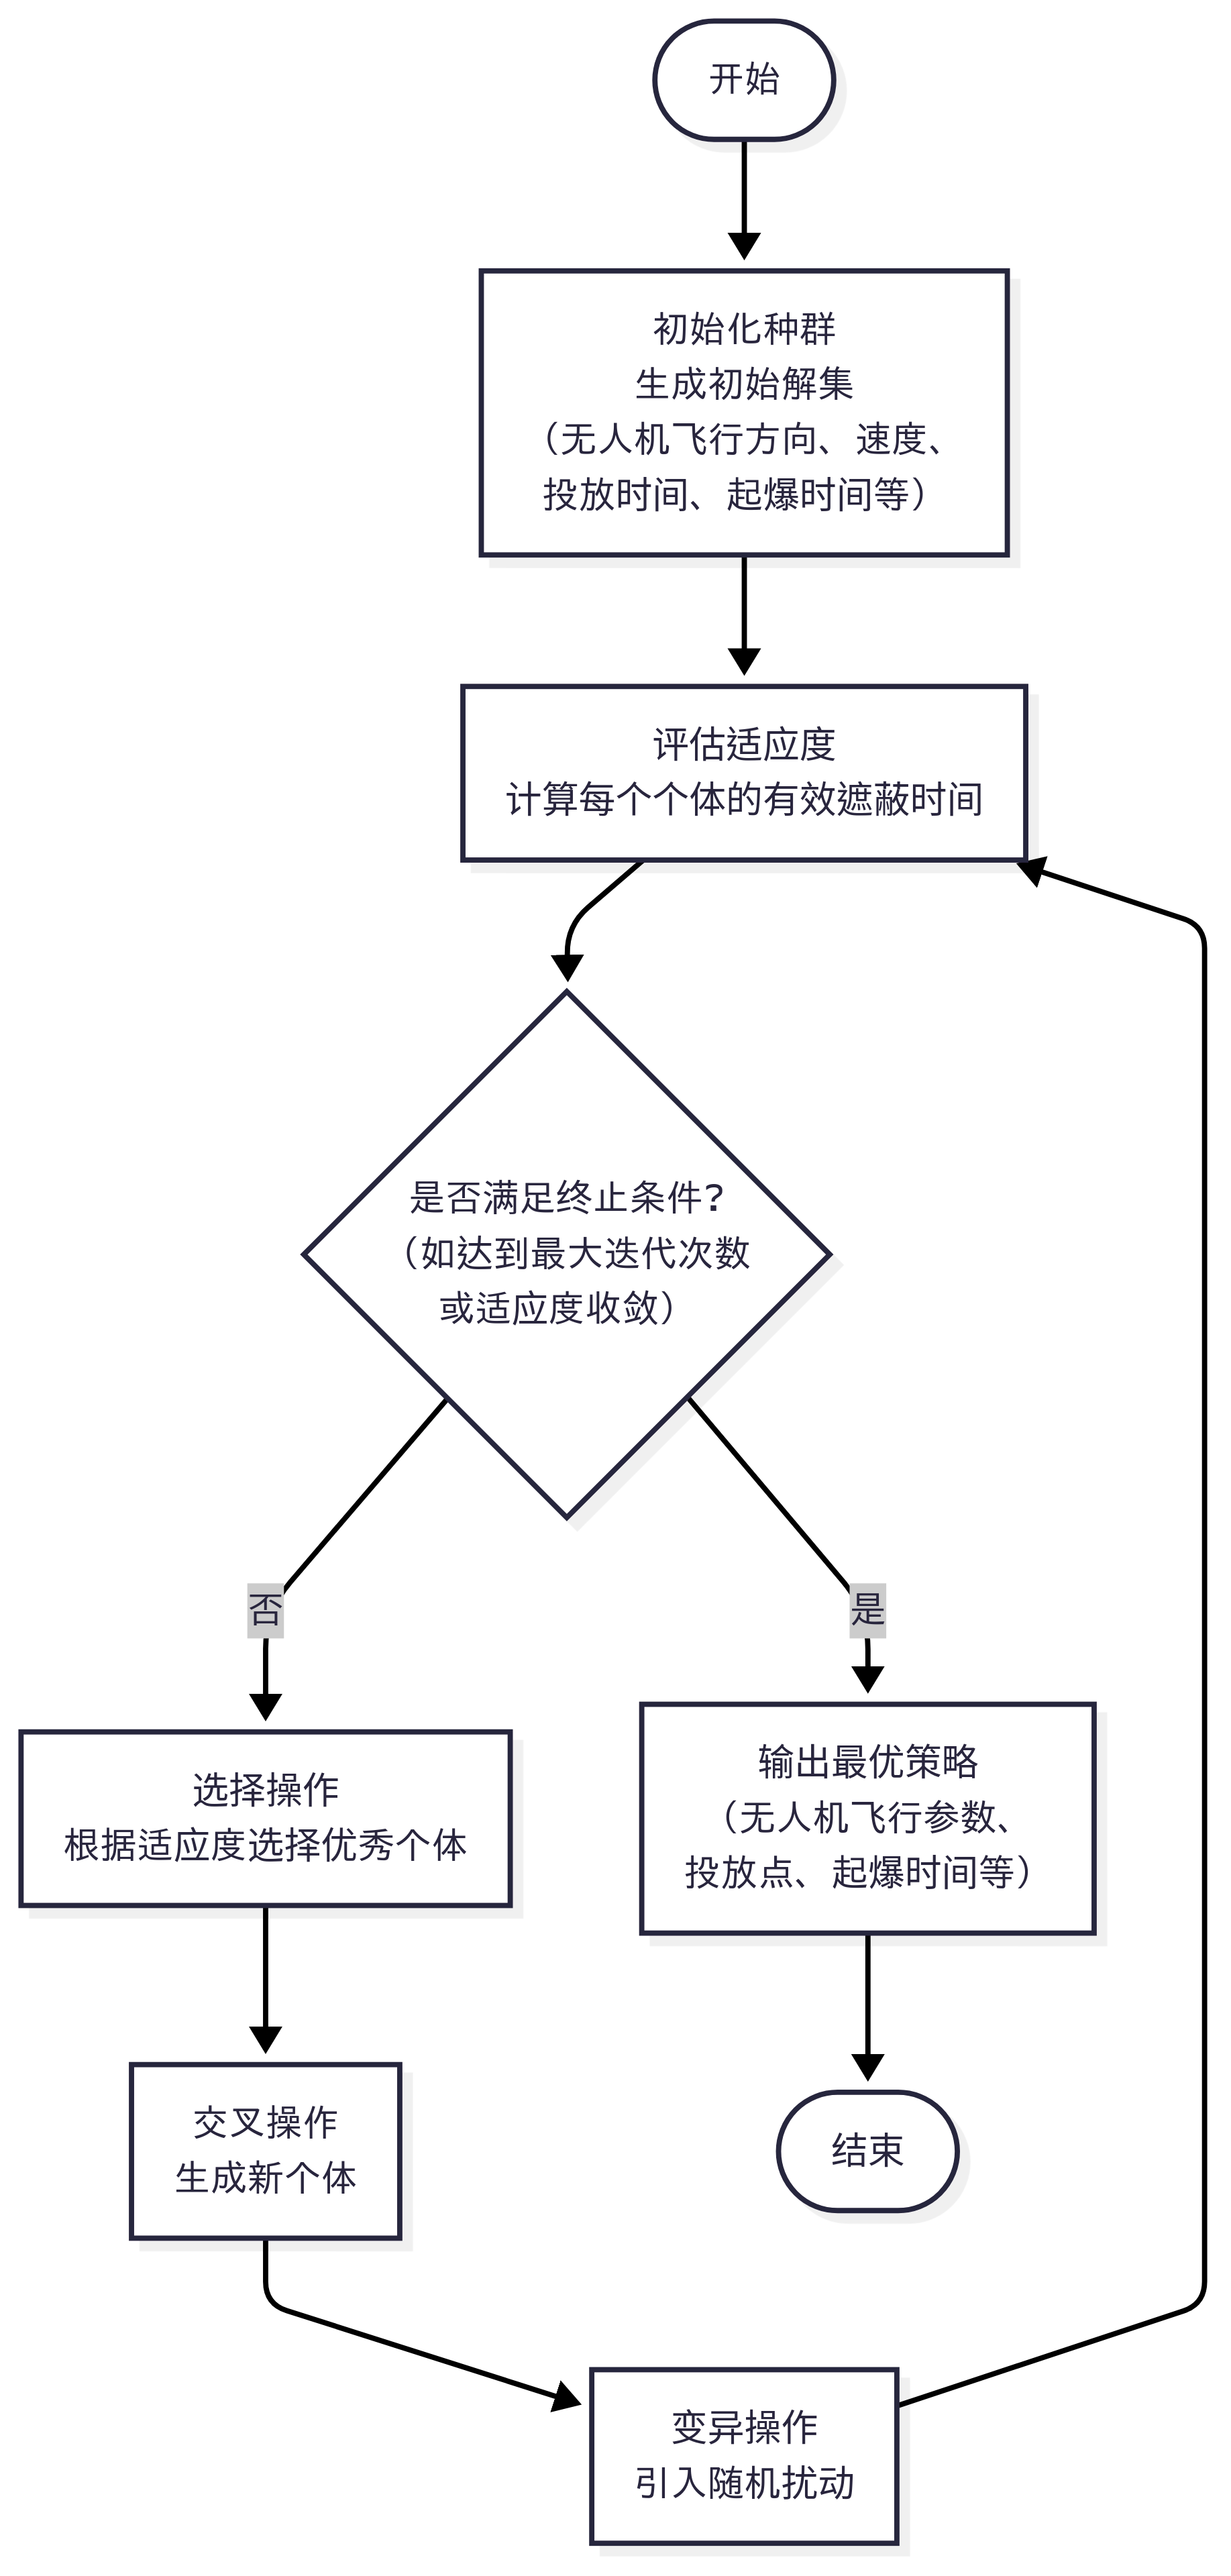
\includegraphics[width=.6\textwidth]{./figures/ga_flowchart}
    \caption{遗传算法流程图}
    \label{fig:ga_flowchart}
\end{figure}

\subsection{问题三分析}

问题三在问题二的基础上，进一步扩展为单架无人机投放三枚烟幕干扰弹，目的是通过合理设计三次投放与起爆时序，使得总的有效遮蔽时间最长。与单弹优化不同，这里不仅需要确定无人机的飞行方向，飞行速度，还要设计三枚烟幕干扰弹的投放时间、间隔时间和起爆时间，以实现三枚烟幕干扰弹遮蔽时间并集的最大化。

由于多个干扰弹的效果具有时间叠加和并集特性，问题三实际上是一个多变量的全局优化问题。笔者采用遗传算法求解：以染色体表示航向角、飞行速度以及三次投放与起爆的参数，适应度函数为三团云雾遮蔽区间的并集时长。为提高效率，算法先用快速几何判据进行可行性筛选，再用严格判据进行高精度评估。这样既能保证搜索速度，又能在复杂的参数空间中逼近最优的多弹投放策略。

\subsection{问题四分析}

问题4在前面单机场景的基础上，引入了多无人机协同：共有三架无人机(FY1、FY2、FY3)，每架各投放一枚烟幕干扰弹，对导弹M1进行联合干扰。与问题2、问题3的单机优化不同，这里每架无人机都有独立的初始位置和可调参数，需要分别确定飞行方向、飞行速度、投放时刻和延时起爆。

建模思路是将问题分解为三个独立的 \textbf{单机优化子问题}：先用遗传算法分别为FY1、FY2、FY3求解单弹最优投放方案，再将结果汇总，输出三机的运动参数，投放点与起爆点坐标以及对应的有效干扰时长。最终结果上三枚烟幕干扰弹的遮蔽时段刚好错开，三个最优解之和一定为全局最优解。这种“分而治之”的方法避免了直接在高维搜索空间中进行全局优化，降低了计算复杂度，同时能保证每架无人机都尽可能发挥最大作用，最终的遮蔽时间由三者的贡献叠加而成。

\subsection{问题五分析}

问题五在问题三和问题四的基础上，要求使用五架无人机(FY1、FY2、FY3、FY4、FY5)各自配备三枚烟幕干扰弹来联合干扰三枚导弹（M1、M2、M3）。不同于前面的问题，问题五的目标函数不能由一个导弹的有效遮蔽时间简单确定，面对多枚导弹我们需要考虑各个导弹的威胁程度，哪个无人机适合用来投放烟幕干扰弹阻碍哪个导弹，综合这些因素来对投弹策略进行优化，来最大化三枚导弹有效遮蔽时间并集的长度。

基于遗传算法，问题五中的基因变量包含了五架无人机的航向、速度、三枚烟幕干扰弹的投放时间、引爆时间。过多的基因变量会使遗传算法的计算量陡增、计算时间过长和计算准确度下降，因此我们首先利用贪心算法将问题初步分解为五个独立的单机遮蔽三弹的优化子问题，再将结果汇总处理，不断迭代，使三枚导弹的有效遮蔽时间并集尽可能长。

\section{模型假设与符号说明}

\subsection{模型假设}

\textbf{1 导弹运动轨迹假设：}导弹朝假目标以定速度300m/s定飞行方向飞行，导弹的飞行轨迹是一条定直线，可以精准地用参数方程表示。

\textbf{2 无人机运动轨迹假设：}无人机在指定位置接受任务后可以立即起飞，起飞时确定飞行方向，与飞行速度（速度范围为70-140m/s），且只能登高飞行，飞行方向与速度一经确定便不再改变。无人机的飞行轨迹是平行于xy平面的定直线，可以精准地用参数方程表示。

\textbf{3 烟幕干扰弹投弹运动假设：}烟幕干扰弹从无人机上投放后做平抛运动，水平方向上继承无人机的飞行速度，竖直方向上仅受重力作用，忽略空气阻力。

\textbf{4 球状烟雾云团假设：}假设烟雾干扰弹起爆后瞬间产生半径为10m的球状烟雾云团，云团一经形成便立即有遮蔽效果。球状烟雾云团形成后便以3m/s匀速下沉，下沉过程中形状不变仍然保持球状，且半径不变，在整个球状烟雾范围内一直有遮蔽效果，直到起爆后20s后完全消散，不再具有任何遮蔽效果。

\textbf{5 有效遮蔽的定义：}在问题1到问题5中，用极小的步长遍历圆柱体的侧面与上顶面，并且对所有点实施是否有效遮蔽检测，即验证是否导弹与圆柱体上每一个点的连线，均与球状烟雾相交。只有满足所有点均被遮蔽才认为真目标被遮蔽。

\textbf{6 真实目标假设：}根据题目描述，真实目标是一个底面半径为7m，高为10m的圆柱体。

\textbf{7 投弹时间间隔假设：}根据题目描述，同一架无人机投放的每两枚烟雾干扰弹的投弹时间间隔需大于等于1s，且每架无人机都可以精准控制其投弹时间。

\textbf{8 起爆时间假设：}假设起爆时间一到，烟雾干扰弹便可以立即爆炸产生球状烟雾，达到遮蔽效果，起爆时间不得晚于烟雾干扰弹平抛运动落地时刻。

\textbf{9 遮蔽效果假设：}假设多枚烟雾干扰弹产生的球状烟雾可以配合实现对一枚或多枚导弹遮蔽视线的效果，一枚干扰弹产生的球状烟雾也可以对多枚导弹产生遮蔽作用。

\textbf{10 计算时间假设：}假设无人机出发前确定飞行方向、飞行速度，烟幕干扰弹投放点和烟幕干扰弹起爆点的计算思考时间无限快，即认为经过思考时间后，导弹的各个参数以及位置不变，排除因计算时间导致的导弹位置的变化，避免计划跟不上变化。

\subsection{符号说明}
            
\setlength{\LTpre}{6pt}   % 可选：长表格前后间距
\setlength{\LTpost}{6pt}

\begin{longtable}{c p{0.55\textwidth} c}
	\caption{符号说明}\label{tab:001}\\
	\hline
	符号 & 说明 & 单位 \\
	\hline
	\endfirsthead
	
	\multicolumn{3}{r}{续表~\ref{tab:001}}\\
	\hline
	符号 & 说明 & 单位 \\
	\hline
	\endhead
	
	\hline
	\multicolumn{3}{r}{接下页}\\
	\endfoot
	
	\hline
	\endlastfoot
	
	$g$ & 重力加速度 & m/s$^{2}$ \\
	\hline
	$v_{\text{missile}}$ & 导弹的速度 & m/s \\
	\hline
	$v_{\text{cloud}}$ & 云团下沉速度 & m/s \\
	\hline
	$v_{\text{drone}}$ & 无人机的速度 & m/s \\
	\hline
	$v_{\min}$ & 无人机飞行最低速度 & m/s \\
	\hline
	$v_{\max}$ & 无人机飞行最高速度 & m/s \\
	\hline
	$R_{\text{effective}}$ & 有效遮蔽半径 & m \\
	\hline
	$T_{\text{effective}}$ & 有效遮蔽时间窗长度 & s \\
	\hline
	interval & 最短投弹时间间隔 & s \\
	\hline
	$T_{\text{end}}$ & 导弹到达假目标时刻 & s \\
	\hline
	$t_{\text{drop}}$ & 无人机投弹时间 & s \\
	\hline
	delay & 干扰弹从投放到爆炸的延时 & s \\
	\hline
	$t_{\text{burst}}$ & 干扰弹爆炸时刻 & s \\
	\hline
	$P_{\text{burst}}$ & 干扰弹爆炸位置 & m \\
	\hline
	$M_i^{0}$ & 导弹 $i$ 在初始时刻的位置 & m \\
	\hline
	$FY_i^{0}$ & 无人机 $i$ 在初始时刻的位置 & m \\
	\hline
	$M_i^{t}$ & 导弹 $i$ 在 $t$ 时刻的位置 & m \\
	\hline
	$FY_i^{t}$ & 无人机 $i$ 在 $t$ 时刻的位置 & m \\
	\hline
	fake & 假目标的位置 & m \\
	\hline
	real & 真目标圆柱底面中心 & m \\
	\hline
	$R$ & 真目标圆柱的半径 & m \\
	\hline
	$H$ & 真目标圆柱的高度 & m \\
	\hline
	PopSize & 遗传算法设定的种群大小 & \\
	\hline
	nGen & 遗传算法设定的迭代代数 & \\
	\hline
	$\theta$ & FY1 的水平航向角（弧度） & rad \\
	\hline
	$[s_j, e_j]$ & 第 $j$ 个遮蔽时间区间的起止时刻 & s \\
	\hline
	$B$ & 真目标可见表面上的采样点 & m \\
	\hline
	$\alpha$ & 退火因子  &  \\
	\hline
	$t_{\text{rel}}^{(k)}$ & 第 $k$ 枚干扰弹的投放时刻 & s \\
	\hline
	$\text{delay}^{(k)}$ & 第 $k$ 枚干扰弹的延时 & s \\
	\hline
	$t_{\text{burst}}^{(k)}$ & 第 $k$ 枚干扰弹的起爆时刻 & s \\
	\hline
	$P_{\text{burst}}^{(k)}$ & 第 $k$ 枚干扰弹的起爆位置 & m \\
	\hline
	$[s_j^{(k)},\,e_j^{(k)}]$ & 第 $k$ 枚弹的遮蔽时间区间 & s \\
	\hline
	$\mathcal{U}$ & 三弹遮蔽区间的并集 & \\
	\hline
	$C(t)$ & 云团中心在 $t$ 时刻的位置 & m \\
	\hline
	$\text{CoverTime}^{(i)}$ & 第 $i$ 架无人机的有效遮蔽总时长 & s \\
	\hline
	$\mathcal{U}_{\text{all}}$ & 三机（FY1–FY3）遮蔽区间的并集 & \\
	\hline
	$\text{CoverTime}_{\text{all}}$ & 三机联合有效遮蔽总时长（并集的测度） & s \\
	\hline
	$T_{\cap}$ & 评估时间上限（由 $T_{\text{end}}$ 与导弹到达时刻综合裁剪所得） & s \\
	\hline
	$\mathcal{U}^{(i)}_{m}$ & 第 $i$ 架无人机对第 $m$ 枚导弹的遮蔽区间并集 &  \\
	\hline
	
	
\end{longtable}
\noindent\textit{注：}凡带上标 \(^{(i)}\) 表示第 \(i\) 架无人机相关量（\(i=1,2,3\)）；凡带上标 \(^{(k)}\) 表示第 \(k\) 枚干扰弹相关量（\(k=1,2,3\)）。


\section{模型的建立与求解}

\subsection{问题一模型的建立与求解}

\subsubsection{模型的建立}

导弹从 $M_1^0$ 进入警戒范围，飞行速度为 $v_{\text{missile}}$ ，方向为“指向 $\mathrm{fake}$ 的单位方向”，导弹一直匀速直线飞行：
\begin{equation}
	M_1^{t}
	=
	M_1^0
	+
	v_{\text{missile}}\;t\;
	\frac{\mathrm{fake}-M_1^0}{\left\|\mathrm{fake}-M_1^0\right\|}\, .
\end{equation}

无人机FY1 等高匀速直线飞行：
\begin{equation}
	FY_1^{t}
	=
	FY_1^0
	+
	v_{\text{drone}}\;t\;
	\frac{\mathrm{fake}-FY_1^0}{\left\|\mathrm{fake}-FY_1^0\right\|}\, ,
\end{equation}

并在 $t_{\text{drop}}$ 投放烟雾干扰弹，经过延时 $\text{delay}$ 起爆，有 $t_{\text{burst}}=t_{\text{drop}}+\text{delay}$。干扰弹在起爆延时内做平抛运动，水平方向速度继承了无人机的速度，竖直方向上只受重力作用，忽略空气阻力。起爆位置
\begin{equation}
	\boxed{
		P_{\text{burst}}
		=
		FY_1^{t_{\text{drop}}}
		+
		v_{\text{drone}}\;\text{delay}\;
		\frac{\mathrm{fake}-FY_1^0}{\left\|\mathrm{fake}-FY_1^0\right\|}
		+
		\big(0,\,0,\,-\tfrac{1}{2}g\,\text{delay}^{2}\big)
	}\, .
\end{equation}

云团以 $v_{\text{cloud}}$ 竖直匀速直线下沉，令
\begin{equation}
	\big(x_c(t),\,y_c(t),\,z_c(t)\big)
	=
	\big(P_{\text{burst},x},\;P_{\text{burst},y},\;P_{\text{burst},z}-v_{\text{cloud}}(t-t_{\text{burst}})\big),
	\quad t\ge t_{\text{burst}} .
\end{equation}

评估时间窗取
\begin{equation}
	t \in \left[\,t_{\text{burst}},\;\min\!\big(t_{\text{burst}}+T_{\text{effective}},\,T_{\text{end}}\big)\,\right].
\end{equation}

遮蔽判据要求严格全覆盖：将真目标（底面中心 $real$、半径 $R$、高度 $H$ 的圆柱体）可见表面离散为采样点集。若在时刻 $t$ 对\textbf{任意采样点} $B$ 均有
\begin{equation}
	\boxed{
		\min_{s\in[0,1]}
		\left\|
		s\,M_1^{t}+(1-s)\,B-\big(x_c(t),y_c(t),z_c(t)\big)
		\right\|
		\;\le\;
		R_{\text{effective}}
	}\, ,
\end{equation}

即表示导弹到圆柱体表面上任意一点B的直线均与球状烟雾相交，则判定真目标在该时刻被\textbf{完全遮蔽}。

\begin{figure}[!h]
    \centering
    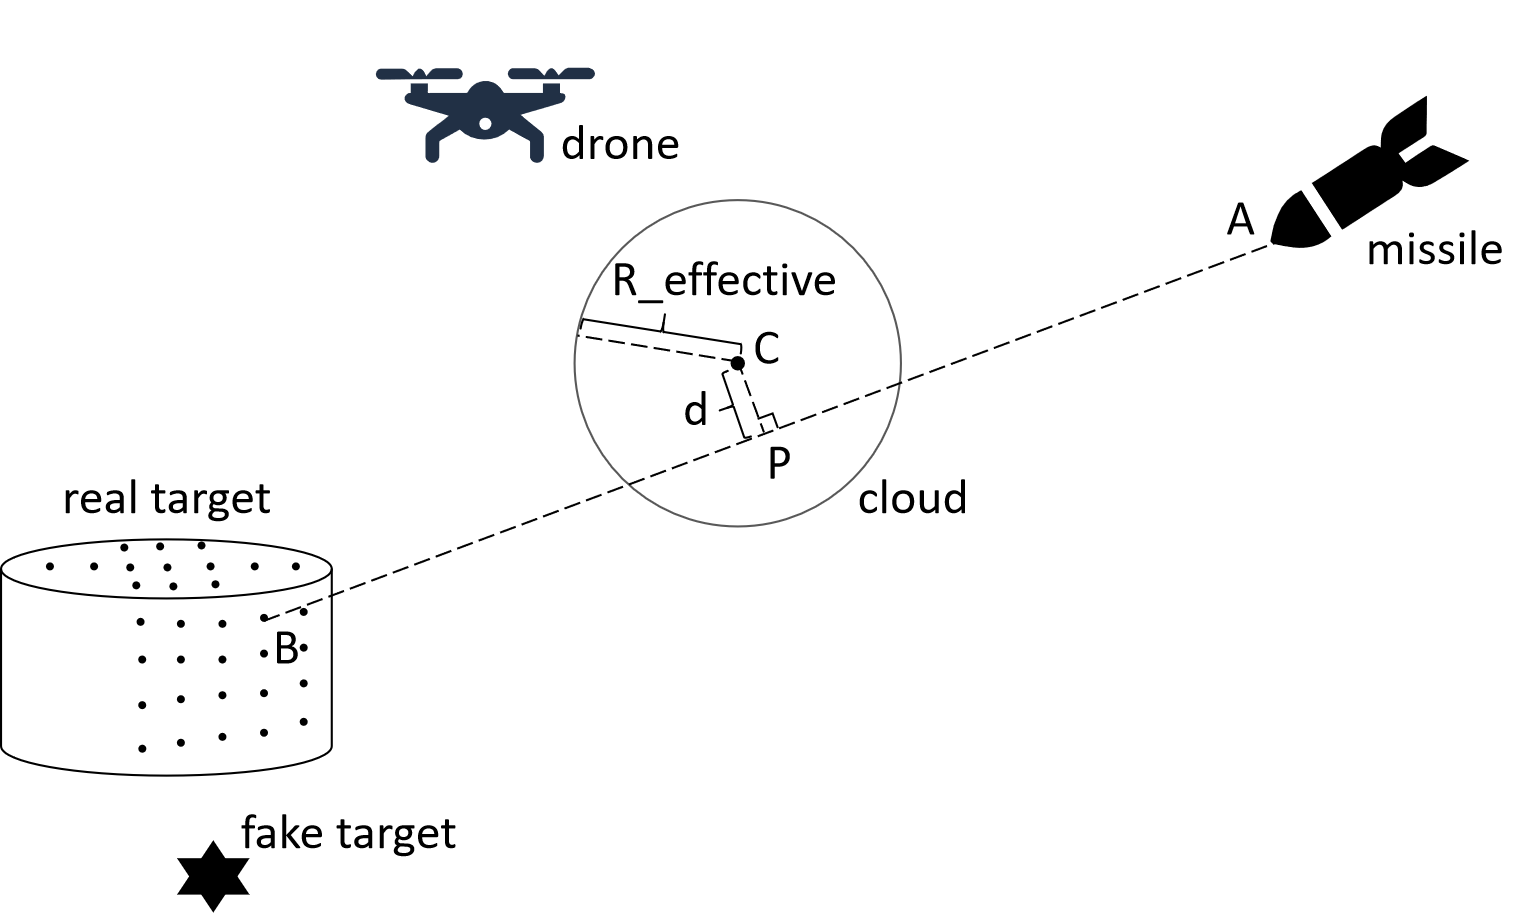
\includegraphics[width=\textwidth]{./figures/precise_criterion}
    \caption{精确判据推导}
    \label{fig:precise_criterion}
\end{figure}

但是这个判据的缺点是计算量较大。为加速计算，可先用快速判据预筛。

快速判据的几何解释为：设导弹和云团中心的连线与和云团的切线的夹角为 $\beta$，导弹和圆柱体中心的连线与和圆柱体外接球的切线的夹角为 $\alpha$，导弹和云团中心的连线与导弹和圆柱体中心的连线的夹角为 $\theta$。若 $\beta\ge\alpha+\theta$，则导弹到圆柱体上任意一点的连线均与云团相交，真目标被遮蔽。

但是这个判据其实是一个充分不必要条件，就是说，当不满足 $\beta\ge\alpha+\theta$ 时，真目标也可能被遮蔽，因此这个判据只能用来预筛，不能作为最终的判据。

\begin{figure}[!h]
    \centering
    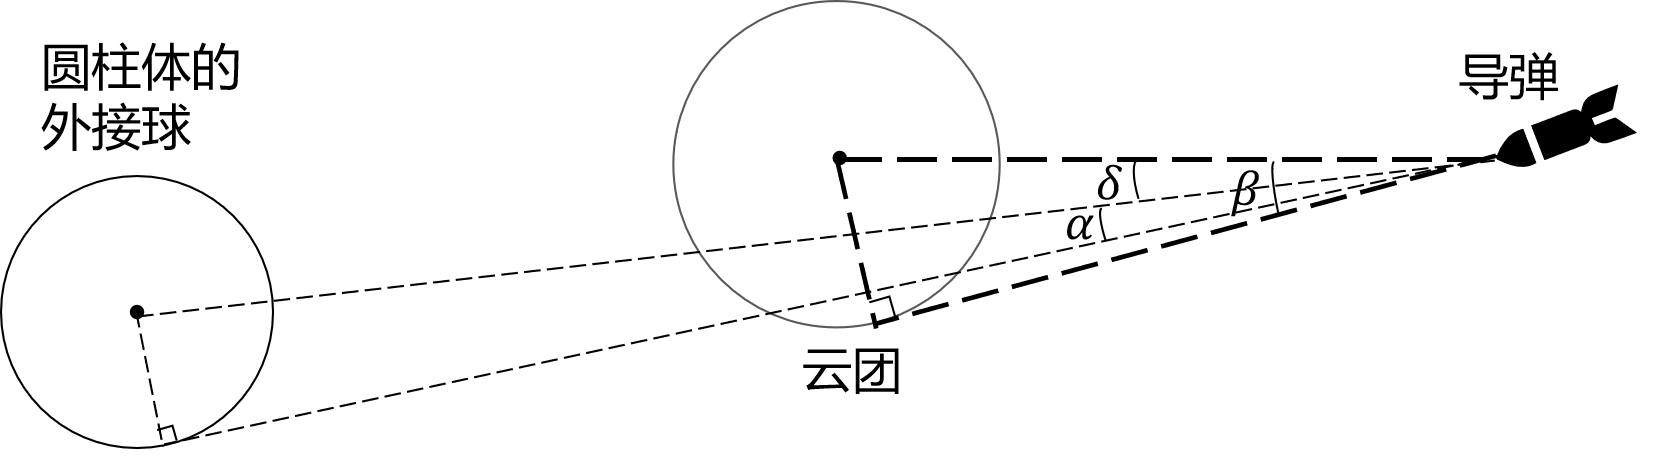
\includegraphics[width=\textwidth]{./figures/quick_criterion}
    \caption{快速判据推导}
    \label{fig:quick_criterion}
\end{figure}

\subsubsection{模型的求解}

(1) 由 $v_{\text{drone}},\,t_{\text{drop}},\,\text{delay}$ 求得 $t_{\text{burst}}$ 与 $P_{\text{burst}}$；

(2) 在 $\left[t_{\text{burst}},\,\min\!\big(t_{\text{burst}}+T_{\text{effective}},\,T_{\text{end}}\big)\right]$ 进行固定步长离散；

(3) 逐时刻计算 $M_1^{t}$ 与 $\big(x_c(t),y_c(t),z_c(t)\big)$，按遮蔽判据检查所有采样点是否均满足 $\le R_{\text{effective}}$，满足则记为\textbf{被遮蔽}；

(4) 合并相邻“被遮蔽”时刻为若干区间 $[s_j,e_j]$，总有效遮蔽时长为
\begin{equation}
	\sum_{j}\big(e_j - s_j\big)\, ;
\end{equation}

(5) 输出 $P_{\text{burst}}$、各区间 $[s_j,e_j]$ 与总时长.

(6) 最终输出为

Burst point (m): x=17188.000, y=0.000, z=1736.431

\textbf{[Total] dur=1.390 }

intervals=[(8.049999999999937, 9.439999999999909)]

\begin{figure}[!h]
    \centering
    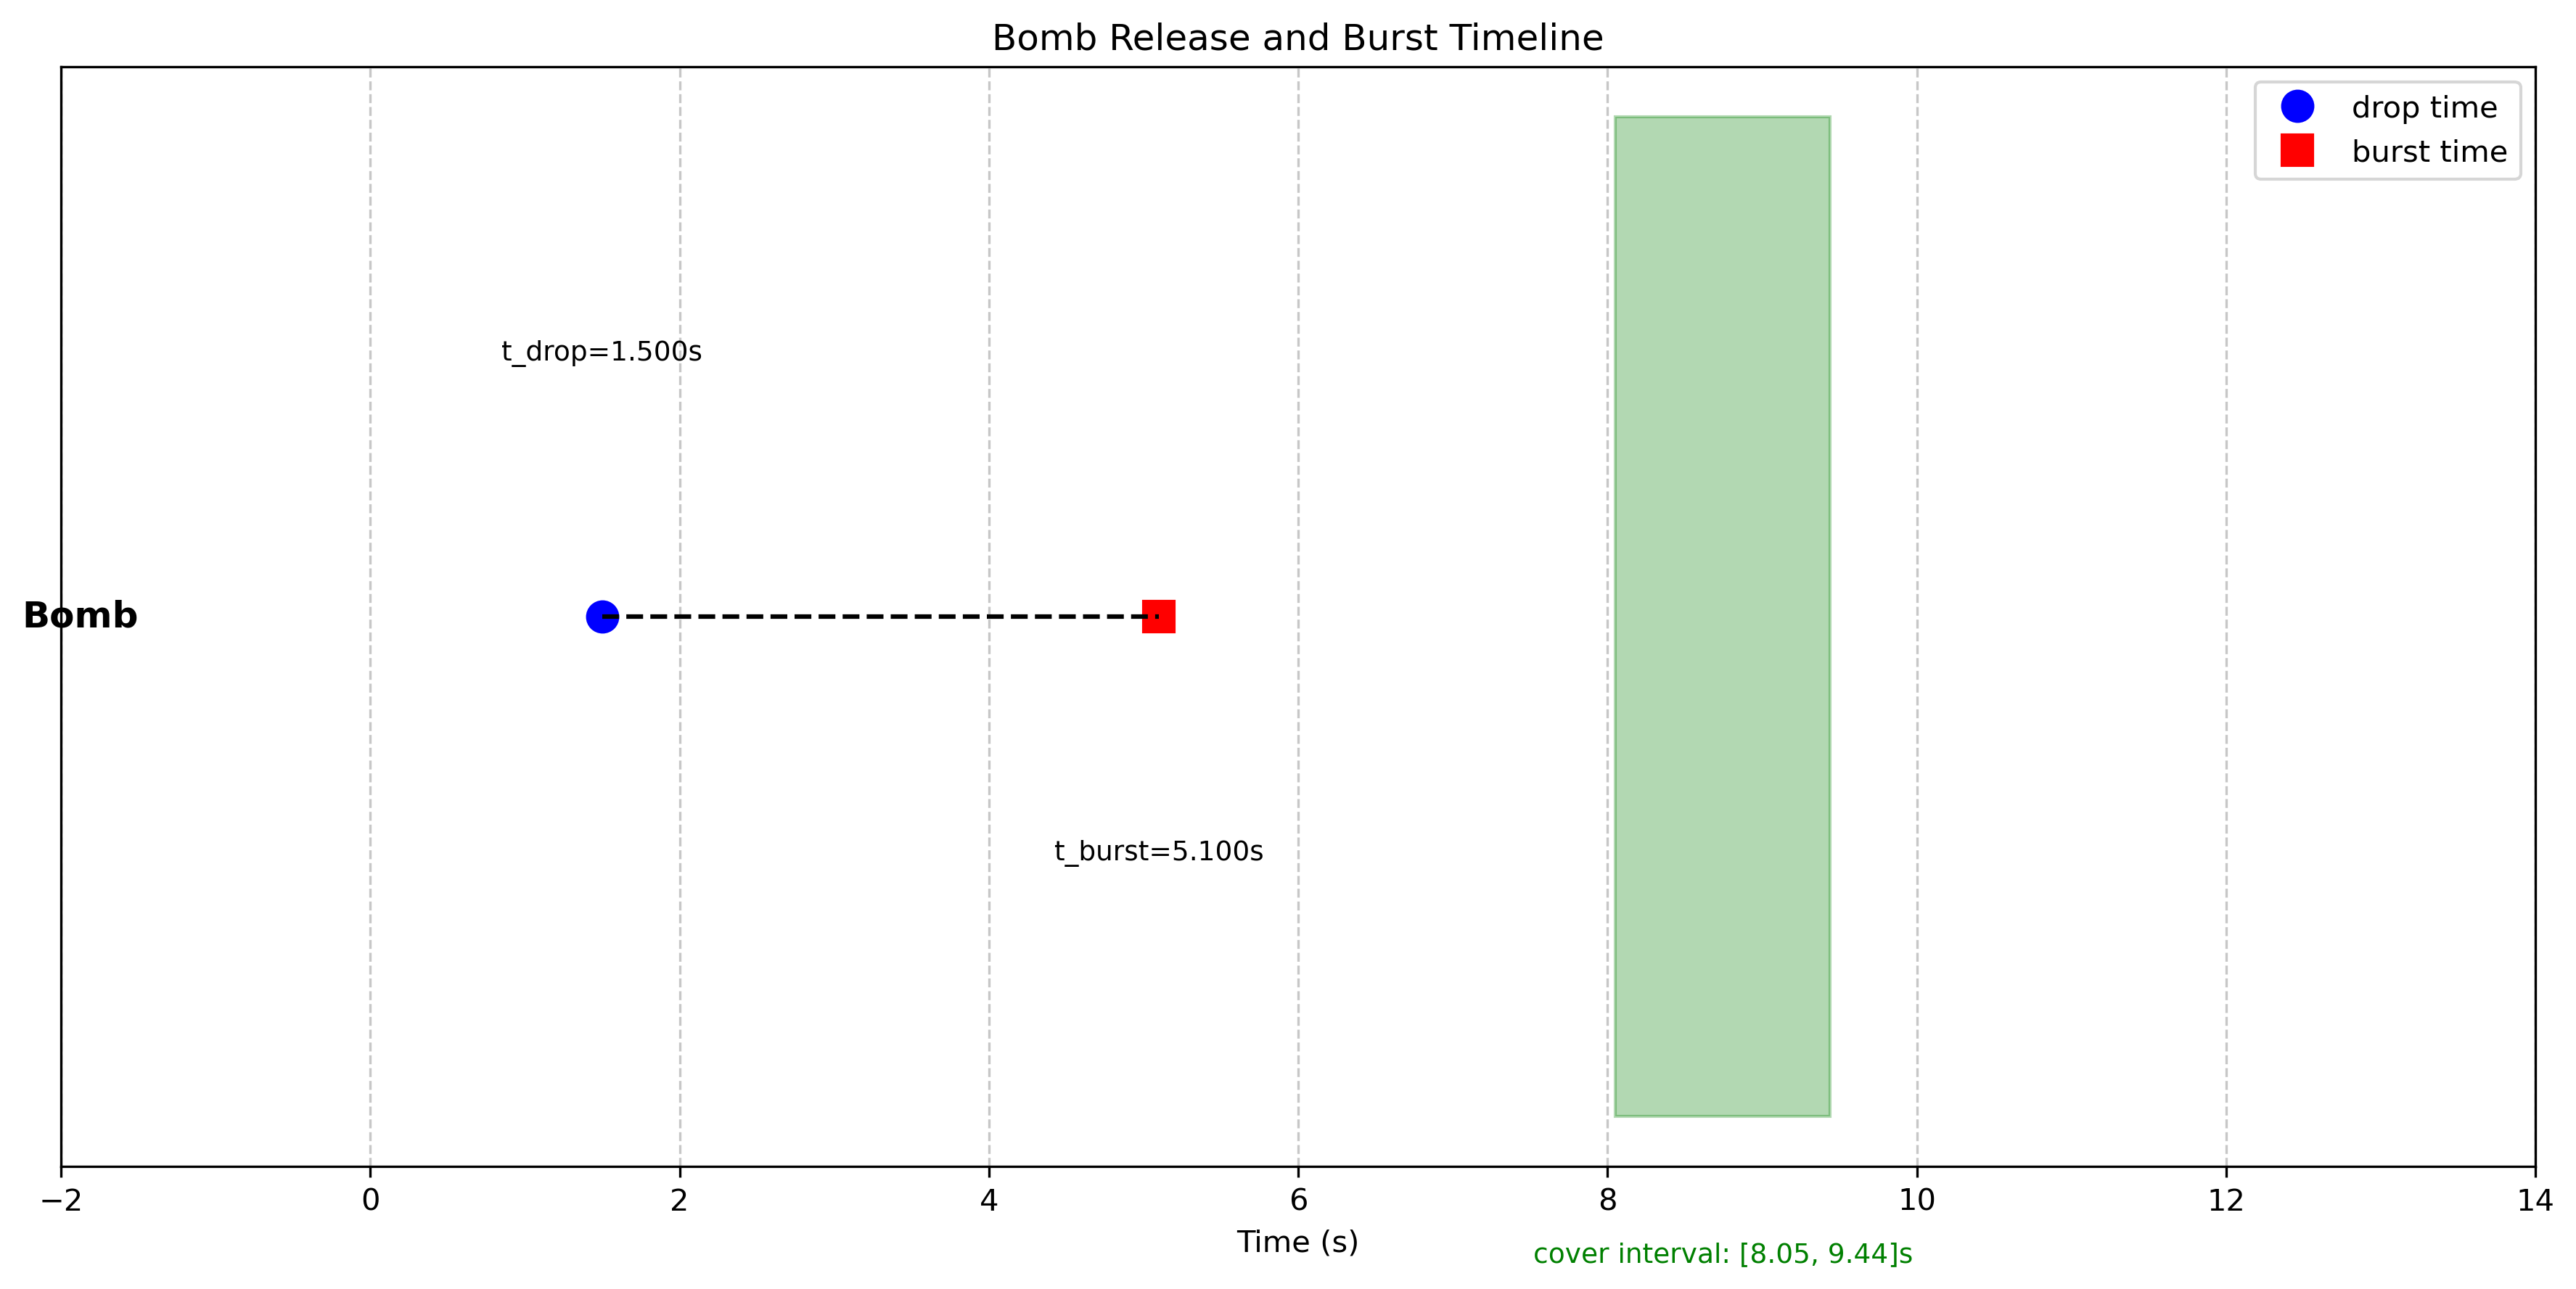
\includegraphics[width=0.8\textwidth]{./figures/bomb_timeline_1}
    \caption{问题1投弹时间线}
    \label{fig:bomb_timeline_1}
\end{figure}

\begin{figure}[!h]
    \centering
    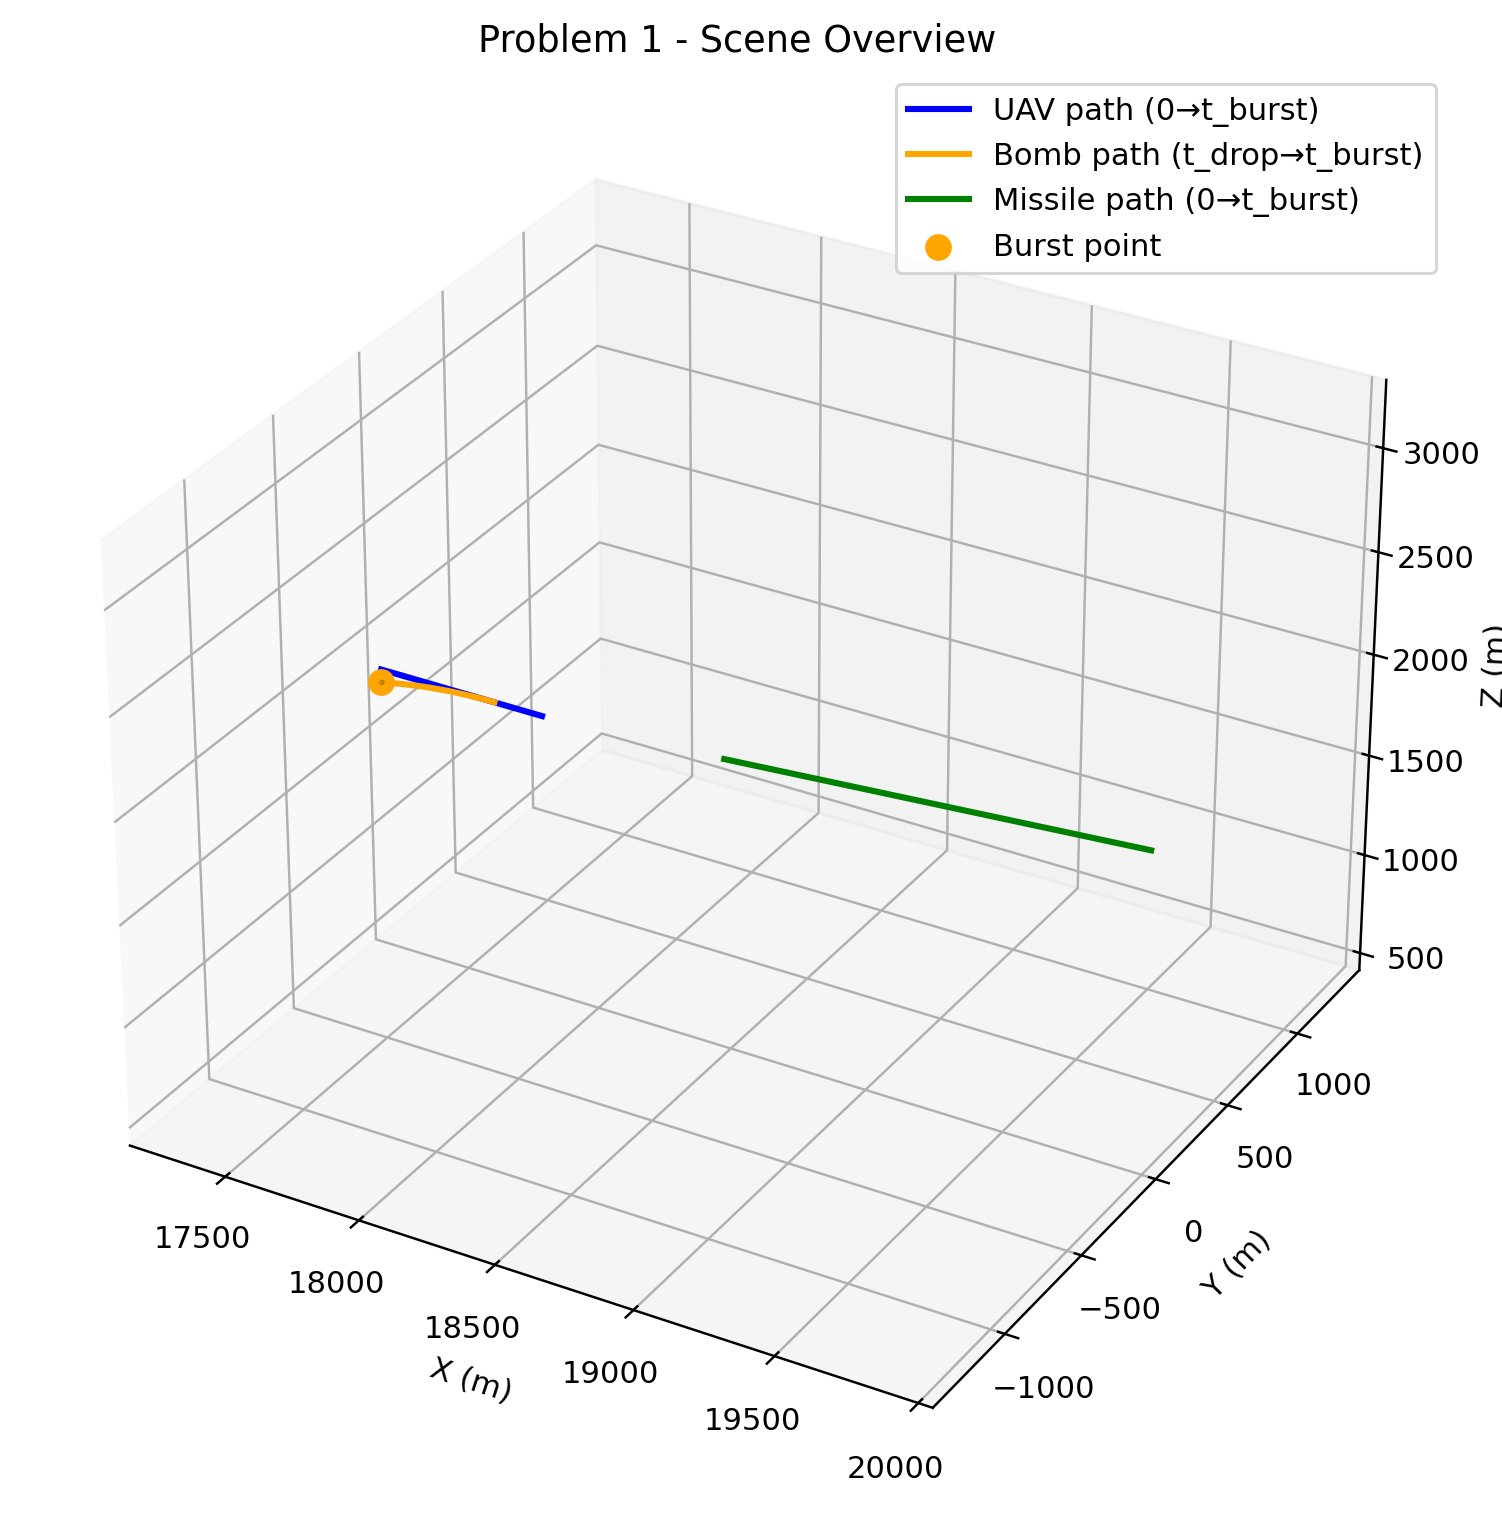
\includegraphics[width=.6\textwidth]{./figures/problem1_3d}
    \caption{问题1的三维场景图}
    \label{fig:problem1_3d}
\end{figure}

\subsection{问题二模型的建立与求解}

\subsubsection{模型的建立}

在单枚干扰弹的设定下，需要寻找最佳的无人机FY1 的水平航向角 $\theta$、飞行速度 $v_{\text{drone}}$、投放时刻 $t_{\text{drop}}$ 与延时起爆 $\text{delay}$，并令
\[
t_{\text{burst}}=t_{\text{drop}}+\text{delay}.
\]
约束条件为
\begin{align}
	v_{\min} &\le v_{\text{drone}} \le v_{\max},\\
	-\pi &\le \theta \le \pi,\\
	0 &\le t_{\text{drop}} \le 30\,\text{s},\\
	0 &\le \text{delay} \le T_{\text{effective}},\\
	t_{\text{burst}} &\le T_{\text{end}}.
\end{align}

对违反 $t_{\text{burst}}\le T_{\text{end}}$ 的情形，进行可行化修复：
\[
\text{delay}\leftarrow \max\!\big(0,\;T_{\text{end}}-t_{\text{drop}}\big),\qquad
t_{\text{burst}}=t_{\text{drop}}+\text{delay}.
\]
\textbf{运动学关系:}

导弹从 $M_1^0$ 出发，以速度 $v_{\text{missile}}$ 指向 $\mathrm{fake}$ 匀速直线飞行：
\begin{equation}
	M_1^{t}
	= M_1^0
	+ v_{\text{missile}}\;t\;
	\frac{\mathrm{fake}-M_1^0}{\left\|\mathrm{fake}-M_1^0\right\|}.
\end{equation}

FY1 等高匀速直线飞行，其水平航向为 $\theta$ ，干扰弹在 $t_{\text{drop}}$ 时刻投放，在 起爆延时$\text{delay}$ 后于 $t_{\text{burst}}$ 起爆。起爆位置为
\begin{equation}
	P_{\text{burst}}
	=
	FY_1^{t_{\text{drop}}}
	+ v_{\text{drone}}\cdot \text{delay}\cdot (\cos\theta,\ \sin\theta,\ 0)
	+ \big(0,\,0,\,-\tfrac12 g\,\text{delay}^2\big).
\end{equation}

起爆后云团以 $v_{\text{cloud}}$ 竖直匀速下沉：
\begin{equation}
	\big(x_c(t),\,y_c(t),\,z_c(t)\big)
	=
	\big(P_{\text{burst},x},\;P_{\text{burst},y},\;P_{\text{burst},z}-v_{\text{cloud}}(t-t_{\text{burst}})\big),
	\quad t\ge t_{\text{burst}},
\end{equation}
并在时间窗
\begin{equation}
	t\in\left[t_{\text{burst}},\ \min\!\big(t_{\text{burst}}+T_{\text{effective}},\ T_{\text{end}}\big)\right]
\end{equation}
内进行评估。

\textbf{遮蔽判据（严格全覆盖）}
将真目标（底面中心 $real$、半径 $R$、高度 $H$ 的圆柱体）可见表面进行离散采样。若在某一时刻 $t$，对每个采样点 $B$ 都有
\begin{equation}
	\min_{s\in[0,1]}
	\left\|
	s\,M_1^{t}+(1-s)\,B
	-\big(x_c(t),y_c(t),z_c(t)\big)
	\right\|
	\ \le\ R_{\text{effective}},
\end{equation}

则判定在 $t$ 时刻被完全遮蔽。对整个时间窗进行逐时刻判定，将收集所有“为真”的时间片段取并集。

\subsubsection{模型的求解}
以\textbf{总有效遮蔽时长为目标}，设所有被遮蔽的时间片段合并为区间 $\{[s_j,e_j]\}$，则本题等价于在满足边界条件与可行化约束的条件下，进行求解
\begin{equation}
	\max_{\,v_{\text{drone}},\,\theta,\,t_{\text{drop}},\,\text{delay}}
	\ \ \sum_{j}\big(e_j-s_j\big)
	\quad
	\text{}
\end{equation}

采用实数编码的遗传算法求解：个体为 $[v_{\text{drone}},\,\theta,\,t_{\text{drop}},\,\text{delay}]$，下界与上界分别为
$[v_{\min},-\pi,0,0]$ 与 $[v_{\max},\pi,30,\,T_{\text{effective}}]$。
解码时计算 $t_{\text{burst}}$ 并执行可行化修复，然后调用问题一的评估内核得到目标值（严格遮蔽判据）。为兼顾效率与精度，采用“两阶段评估”：先以较大的步长进行粗评并预筛个体，再以较小的步长对候选与精英进行严格复评。进化操作包括锦标赛选择、SBX 交叉（$\eta=12.0$、交叉概率 $0.9$）与高斯扰动变异；对基因向量
$[v_{\text{drone}},\,\theta,\,t_{\text{drop}},\,\text{delay}]$
的扰动尺度取
\[
\big[\,0.05\,(v_{\max}-v_{\min}),\ \ 0.06\pi,\ \ 0.6\,\alpha,\ \ 0.5\,\alpha\,\big],
\]

其中 $\alpha$ 为按代数线性递减（不低于 $0.45$）的退火因子。达到迭代上限或收敛阈值后，输出最优
$\big(v_{\text{drone}},\theta,t_{\text{drop}},\text{delay},t_{\text{burst}}\big)$，
并给出对应的 $P_{\text{burst}}$、遮蔽区间 $\{[s_j,e_j]\}$ 及其总长度用于展示与复现。

\begin{figure}[!h]
    \centering
    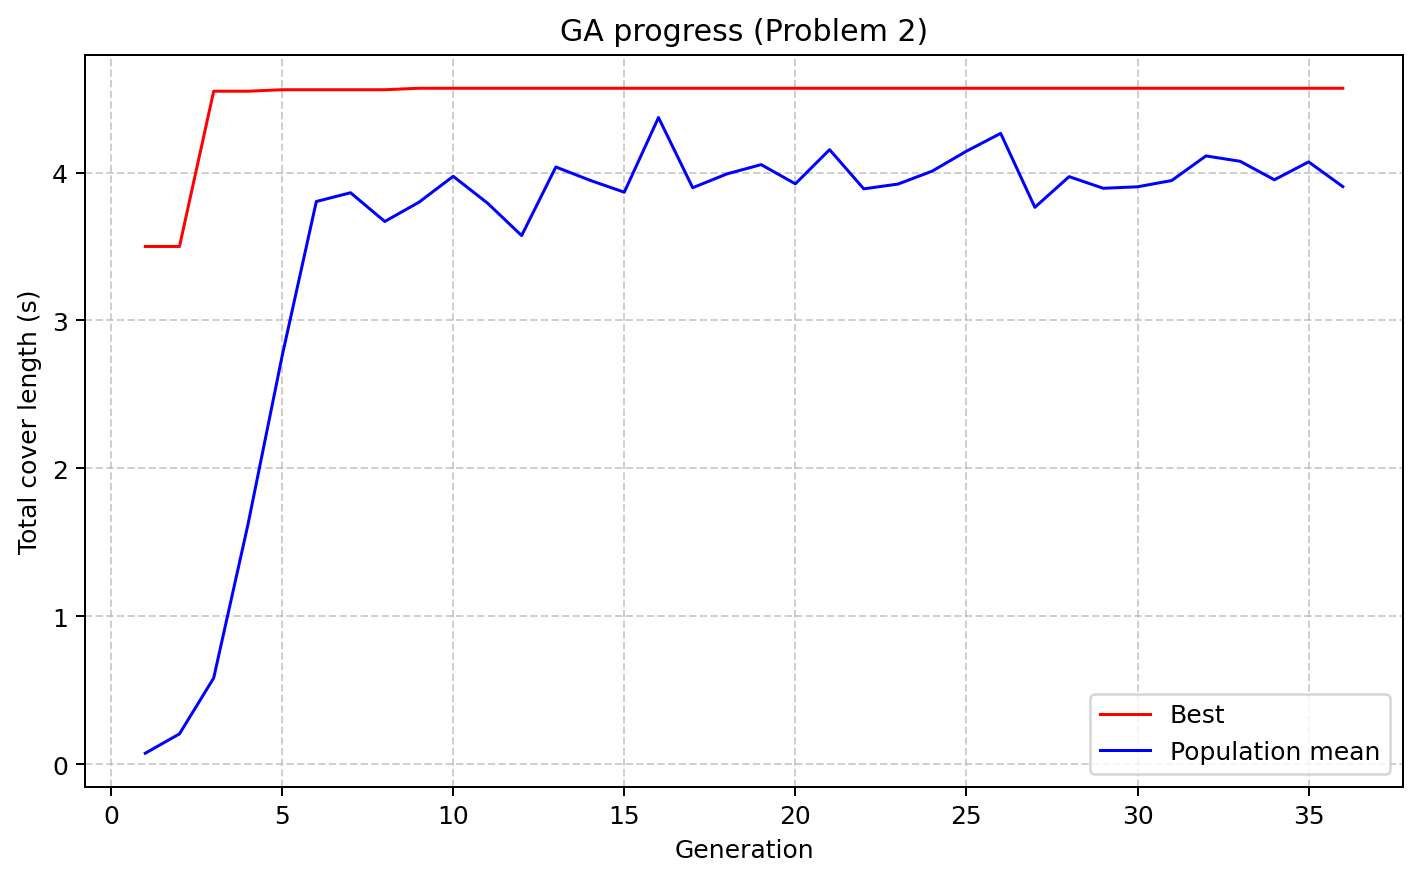
\includegraphics[width=\textwidth]{./figures/problem2_ga_progress}
    \caption{问题2的遗传算法进展图}
    \label{fig:problem2_ga_progress}
\end{figure}

\textbf{最终结果为：}

=== Problem 2 — GA Best Plan (final, total-length objective) ===

\textbf{Total cover length: 4.570 s}

Speed v = 74.623 m/s, Heading θ = 6.371°

Drop time: 0.461 s, 

Delay: 0.793 s, 

Burst: 1.254 s

Burst pos: (17892.987, 10.382, 1796.919) m

Effective cover intervals:

\textbf{Interval 1: 1.540 s to 6.110 s (duration: 4.570 s)}

\begin{figure}[!h]
    \centering
    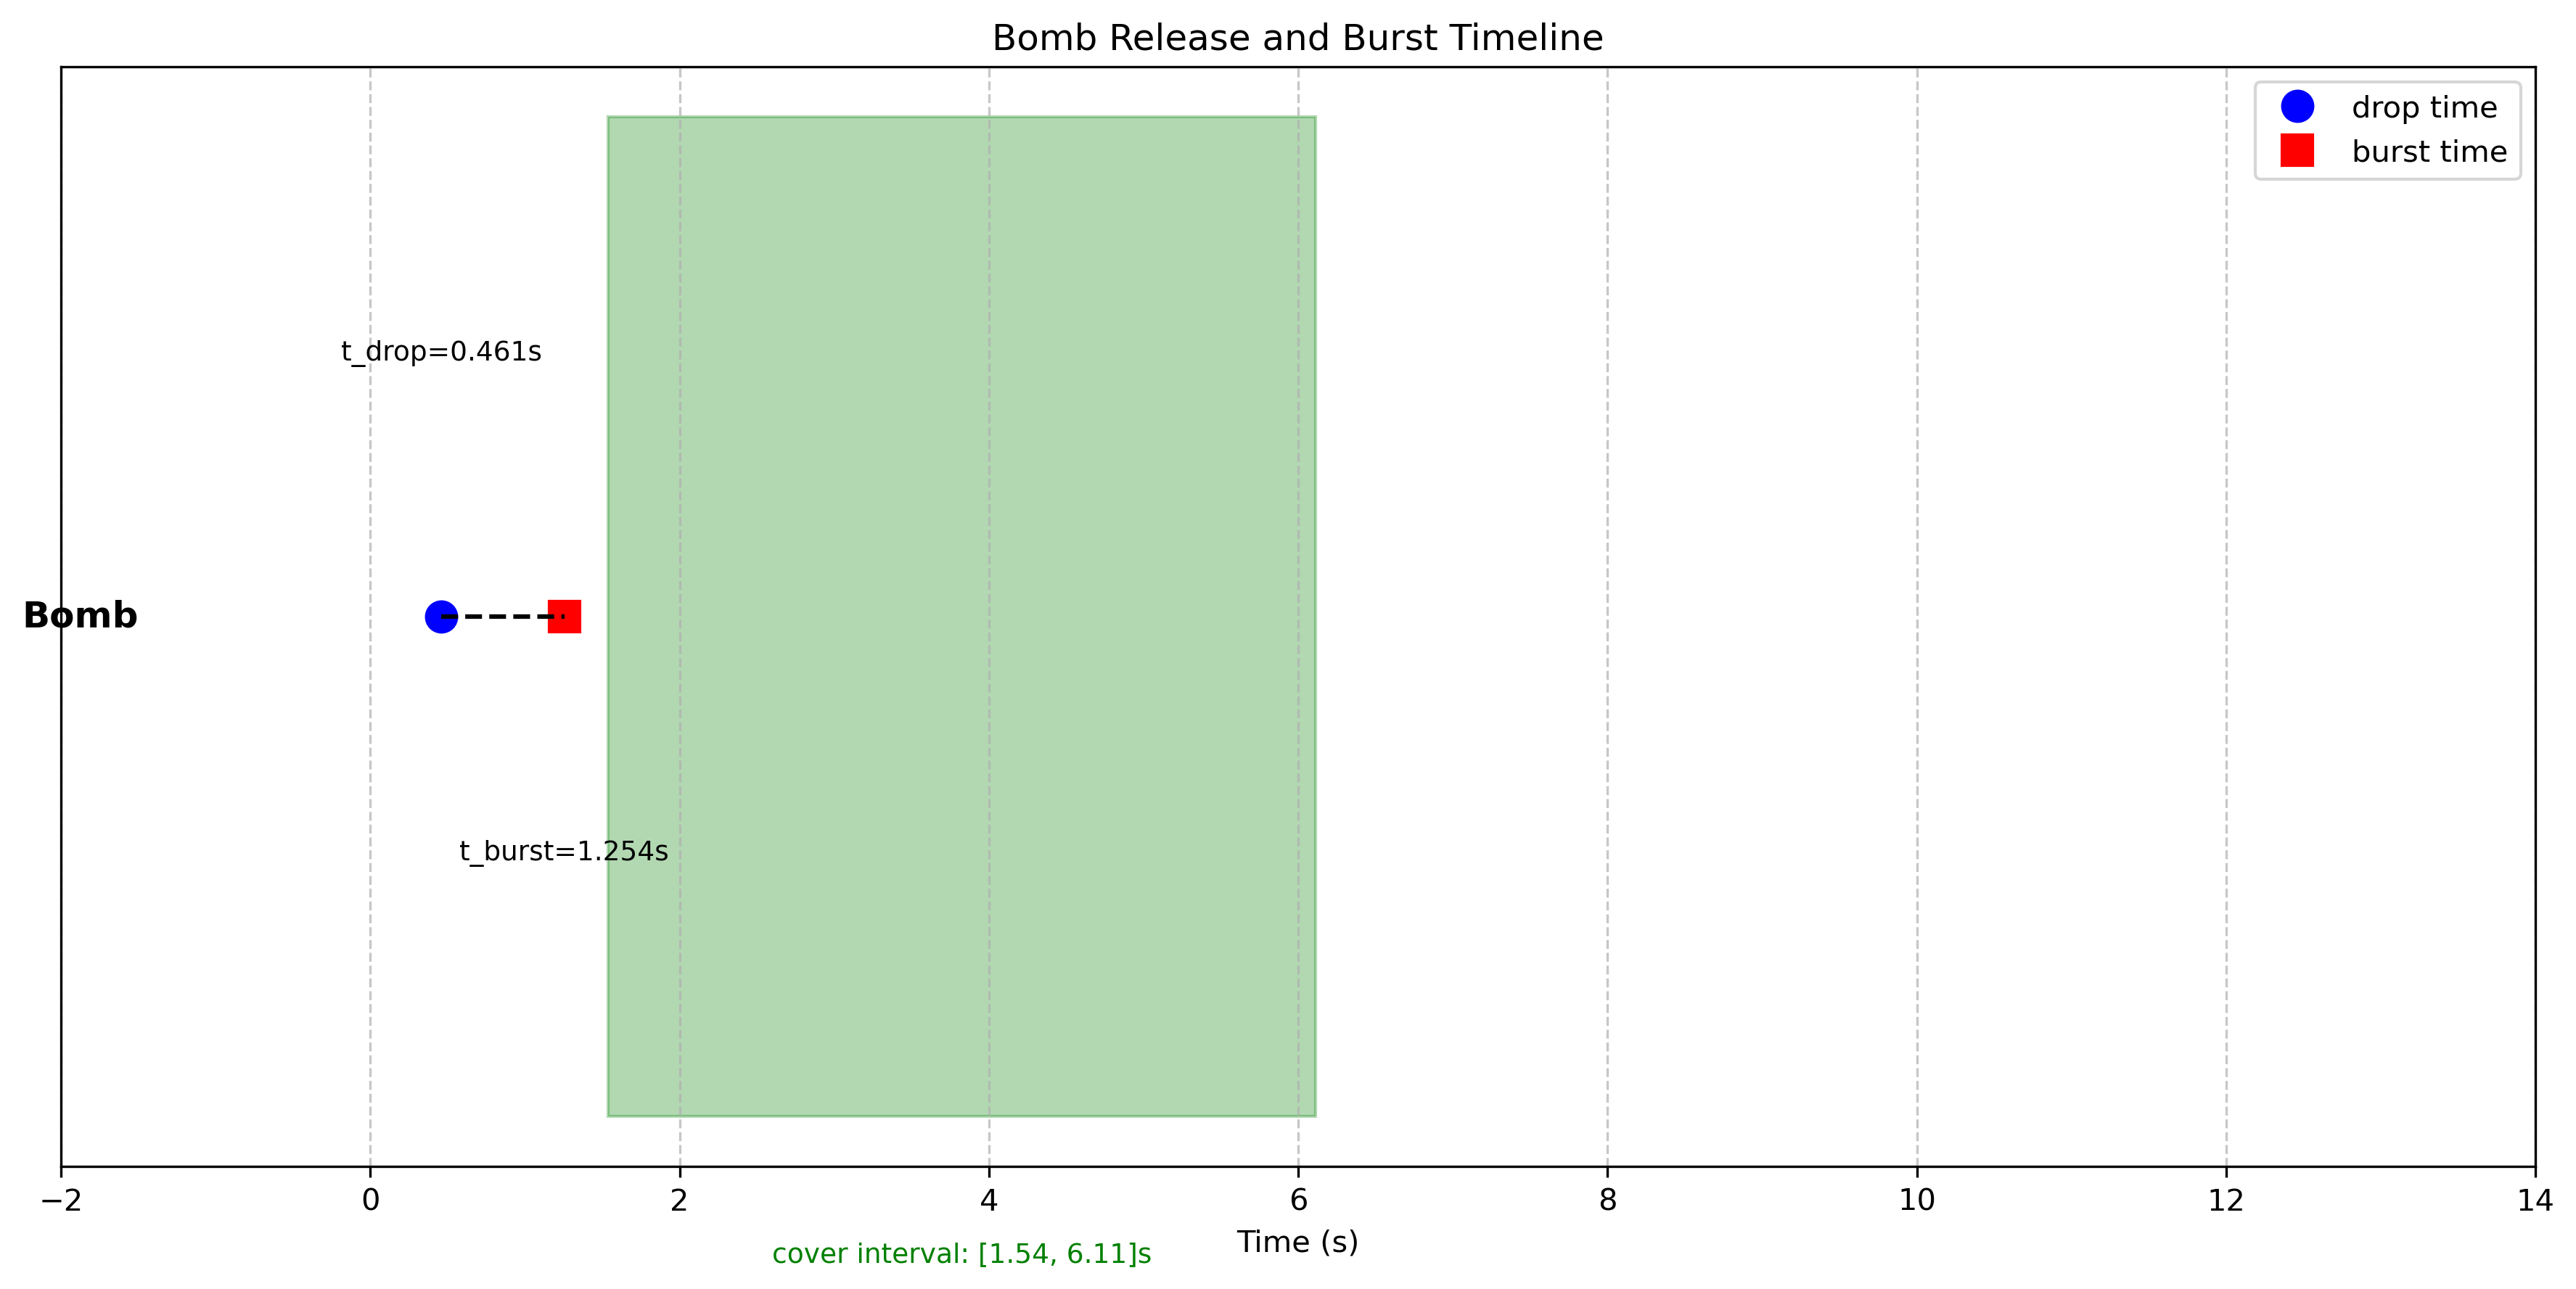
\includegraphics[width=0.8\textwidth]{./figures/bomb_timeline_2}
    \caption{问题2投弹时间线}
    \label{fig:bomb_timeline_2}
\end{figure}

\begin{figure}[!h]
    \centering
    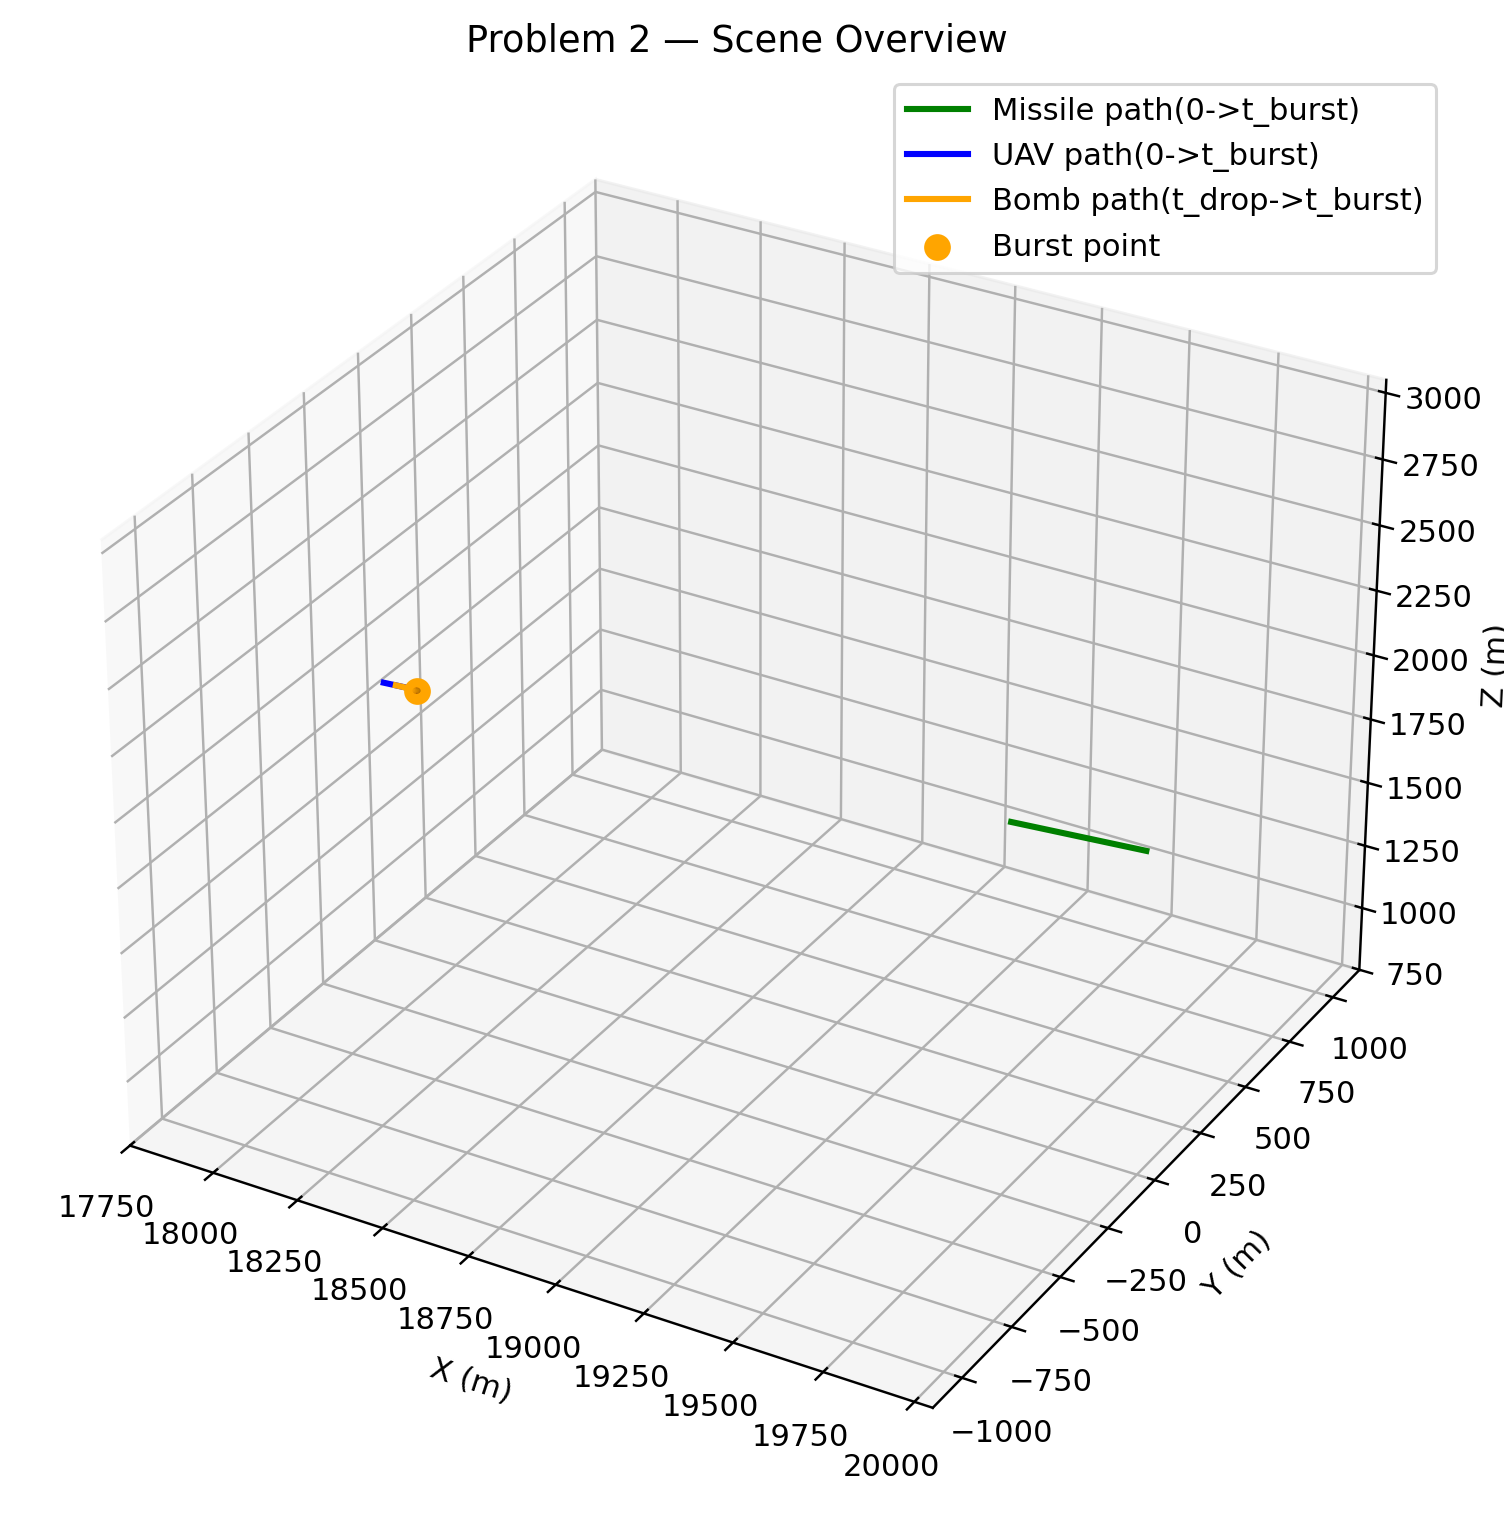
\includegraphics[width=.6\textwidth]{./figures/problem2_3d}
    \caption{问题2的三维场景图}
    \label{fig:problem2_3d}
\end{figure}

\subsection{问题三模型的建立与求解}

\subsubsection{模型的建立}

问题3在只有一架无人机FY1投放三枚干扰弹的条件下，需全局搜索最优的水平航向角 $\theta$、飞行速度 $v_{\text{drone}}$，
以及三枚烟雾干扰弹分别的投弹时间与起爆延时 $\{t_{\text{rel}}^{(k)},\,\text{delay}^{(k)}\}_{k=1}^3$，其中
\[
t_{\text{burst}}^{(k)}=t_{\text{rel}}^{(k)}+\text{delay}^{(k)} .
\]

决策还需要满足下列物理与边界约束：
\begin{align}
	v_{\min} &\le v_{\text{drone}} \le v_{\max},\\
	-\pi &\le \theta \le \pi,\\
	t_{\text{rel}}^{(1)} &\ge 0,\\
	t_{\text{rel}}^{(2)} - t_{\text{rel}}^{(1)} &\ge \text{interval},\\
	t_{\text{rel}}^{(3)} - t_{\text{rel}}^{(2)} &\ge \text{interval},\\
	0 &\le \text{delay}^{(k)} \le 6\,\text{s}\quad (k=1,2,3),\\
	t_{\text{burst}}^{(k)} &= t_{\text{rel}}^{(k)} + \text{delay}^{(k)} \ \le\ T_{\text{end}}\quad (k=1,2,3).
\end{align}

导弹从 $M_1^0$ 出发，以 $v_{\text{missile}}$ 指向 $\mathrm{fake}$ 匀速直线飞行：
\begin{equation}
	M_1^{t}
	= M_1^0
	+ v_{\text{missile}}\;t\;
	\frac{\mathrm{fake}-M_1^0}{\left\|\mathrm{fake}-M_1^0\right\|}.
\end{equation}

无人机FY1 等高直线匀速，水平方向由 $\theta$ 给出。第 $k$ 枚弹在 $t_{\text{rel}}^{(k)}$ 投放，延时 $\text{delay}^{(k)}$ 后于 $t_{\text{burst}}^{(k)}$ 起爆，其起爆位置为
\begin{equation}
	P_{\text{burst}}^{(k)}
	=
	FY_1^0
	+ v_{\text{drone}}\;t_{\text{burst}}^{(k)}\;(\cos\theta,\ \sin\theta,\ 0)
	+ \big(0,\,0,\,-\tfrac12 g\,[\,t_{\text{burst}}^{(k)}-t_{\text{rel}}^{(k)}\,]^2\big).
\end{equation}

起爆后云团以3m/s的速度竖直匀速下沉，且每枚烟雾干扰弹的评估时间窗为
\begin{gather}
	t\in\Big[t_{\text{burst}}^{(k)},\ \min\big(t_{\text{burst}}^{(k)}+T_{\text{effective}},\ T_{\text{end}}\big)\Big],\\
	C^{(k)}(t)=\Big(P_{\text{burst},x}^{(k)},\ P_{\text{burst},y}^{(k)},\ P_{\text{burst},z}^{(k)}-v_{\text{cloud}}\,[\,t-t_{\text{burst}}^{(k)}\,]\Big).
\end{gather}

遮蔽判据沿用问题一的“严格全覆盖”：在任一时刻 $t$，对真目标（底面中心 $real$、半径 $R$、高度 $H$ 的圆柱体）可见表面离散采样。若对每个采样点 $B$ 都有
\begin{equation}
	\min_{s\in[0,1]}
	\left\|\, s\,M_1^{t} + (1-s)\,B \;-\; C^{(k)}(t) \,\right\|
	\ \le\ R_{\text{effective}},
\end{equation}

则判定“第 $k$ 枚弹在时刻 $t$ 形成完全遮蔽”。将满足条件的时刻并为区间集合 $\{[s_j^{(k)},e_j^{(k)}]\}$。

\subsubsection{模型的求解}

三枚弹的遮蔽区间取 \textbf{并集}
\begin{equation}
	\mathcal{U}=\bigcup_{k=1}^{3}\ \bigcup_j [\,s_j^{(k)},\,e_j^{(k)}\,],
\end{equation}

目标是在满足上述边界条件与物理约束的条件下，最大化并集的总长度，即总有效遮蔽时长：
\begin{equation}
	\max_{\;v_{\text{drone}},\,\theta,\,\{t_{\text{rel}}^{(k)},\text{delay}^{(k)}\}_{k=1}^3}
	\ \ \operatorname{len}(\mathcal{U})
	\quad
	\text{}
\end{equation}

求解上采用遗传算法进行连续全局搜索。染色体使用实数编码：
\[
\mathbf{x}=
\bigl[\theta,\ v_{\text{drone}},\ t_{\text{rel}}^{(1)},\ \text{delay}^{(1)},\
t_{\text{rel}}^{(2)},\ \text{delay}^{(2)},\
t_{\text{rel}}^{(3)},\ \text{delay}^{(3)}\bigr].
\]

每个个体在解码阶段被强制满足间隔约束与
\(t_{\text{burst}}^{(k)}\le T_{\text{end}}\ (k=1,2,3)\)，
适应度由严格判据下的区间并集长度给出。

为兼顾效率与精度，采用“粗筛+细筛”的两阶段评估：
先用较大步长进行粗评快速筛选；
再对精英及候选以较小步长进行严格复评，
最终返回最优解及对应的 \(P_{\text{burst}}^{(k)}\) 与并集区间。

\begin{figure}[!h]
    \centering
    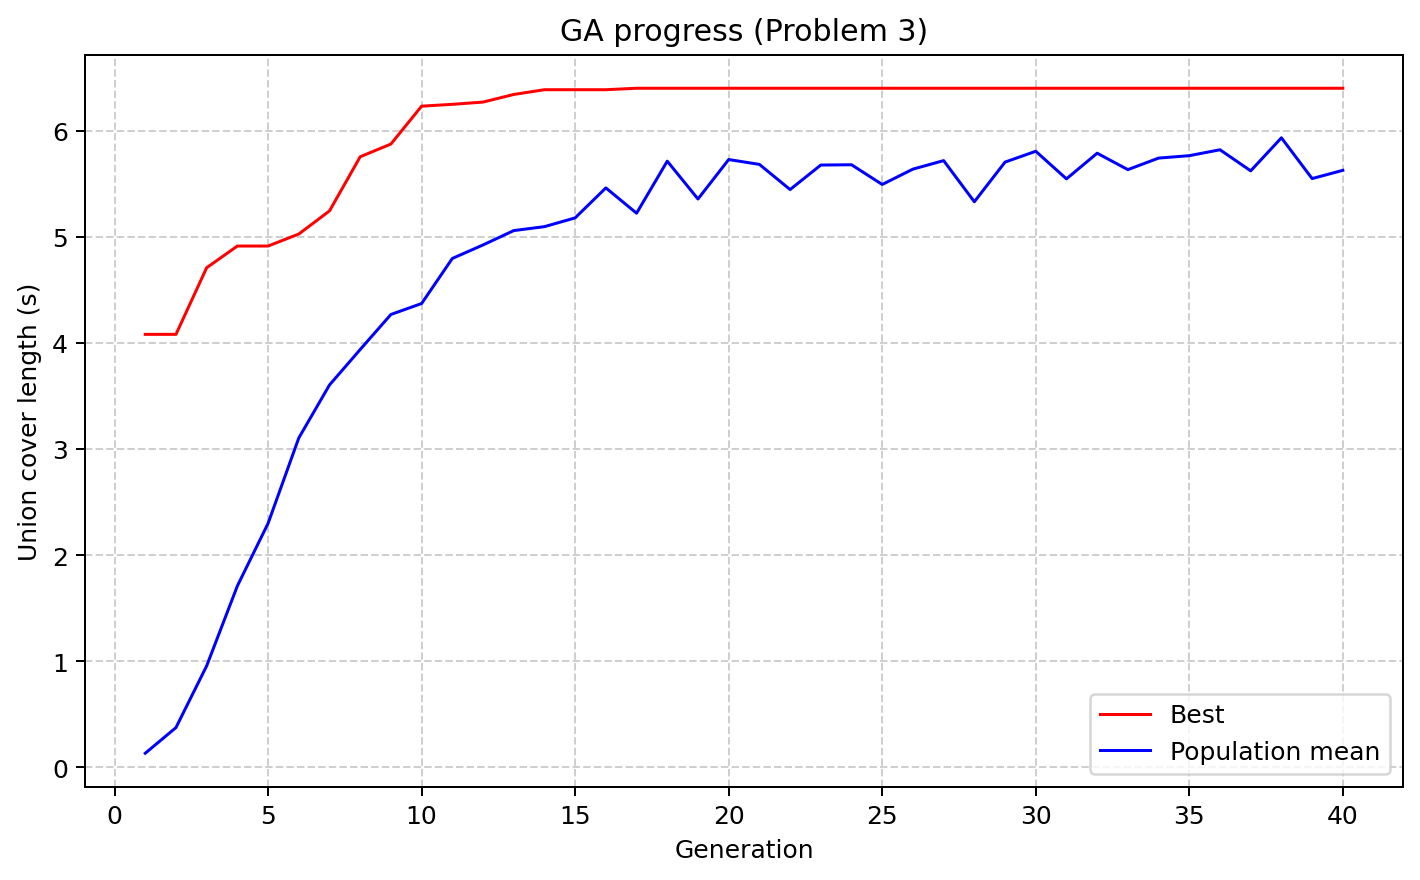
\includegraphics[width=\textwidth]{./figures/problem3_ga_progress}
    \caption{问题3的遗传算法进展图}
    \label{fig:problem3_ga_progress}
\end{figure}

\textbf{最终结果为：}
\begin{table}[h]
	\centering
	\caption{问题三的结果}
	\label{tab:problem3_result}
	\setlength{\tabcolsep}{3.5pt} % 缩小列间距（默认约6pt）
	\small % 也可用 \footnotesize
	\resizebox{\linewidth}{!}{%
		\begin{tabular}{ccccccc}
			\toprule
			烟幕干扰弹编号 & 投放时间 (s) & 投放点坐标 (m) & 起爆时间 (s) &
			起爆点坐标 (m) & 覆盖区间 (s) & 有效遮蔽时间 (s) \\
			\midrule
			弹\#1 & $0.00$ & $(17800.00, 0.00, 1800.00)$ & $0.00$ &
			$(17800.00, 0.00, 1800.00)$ & $[(4.85,\,7.4)]$ & $2.55$ \\
			弹\#2 & $1.00$ & $(17937.12, 11.89, 1800.00)$ & $1.00$ &
			$(17937.12, 11.89, 1800.00)$ & $[(1.0,\,5.37)]$ & $4.37$ \\
			弹\#3 & $2.86$ & $(18192.04, 33.99, 1800.00)$ & $4.12$ &
			$(18365.23, 49.01, 1792.18)$ & $[\ ]$ & $0.00$ \\
			\bottomrule
		\end{tabular}%
	}
\end{table}

\textbf{问题三总体参数：} \begin{itemize} \item 无人机航向 = 4.96°，速度 = 137.6 m/s \item 
	\textbf{三团烟雾干扰时间并集（严格）= 6.400 s} \item 并集区间 = $[(1.0, 7.4)]$ \end{itemize}

\begin{figure}[!h]
    \centering
    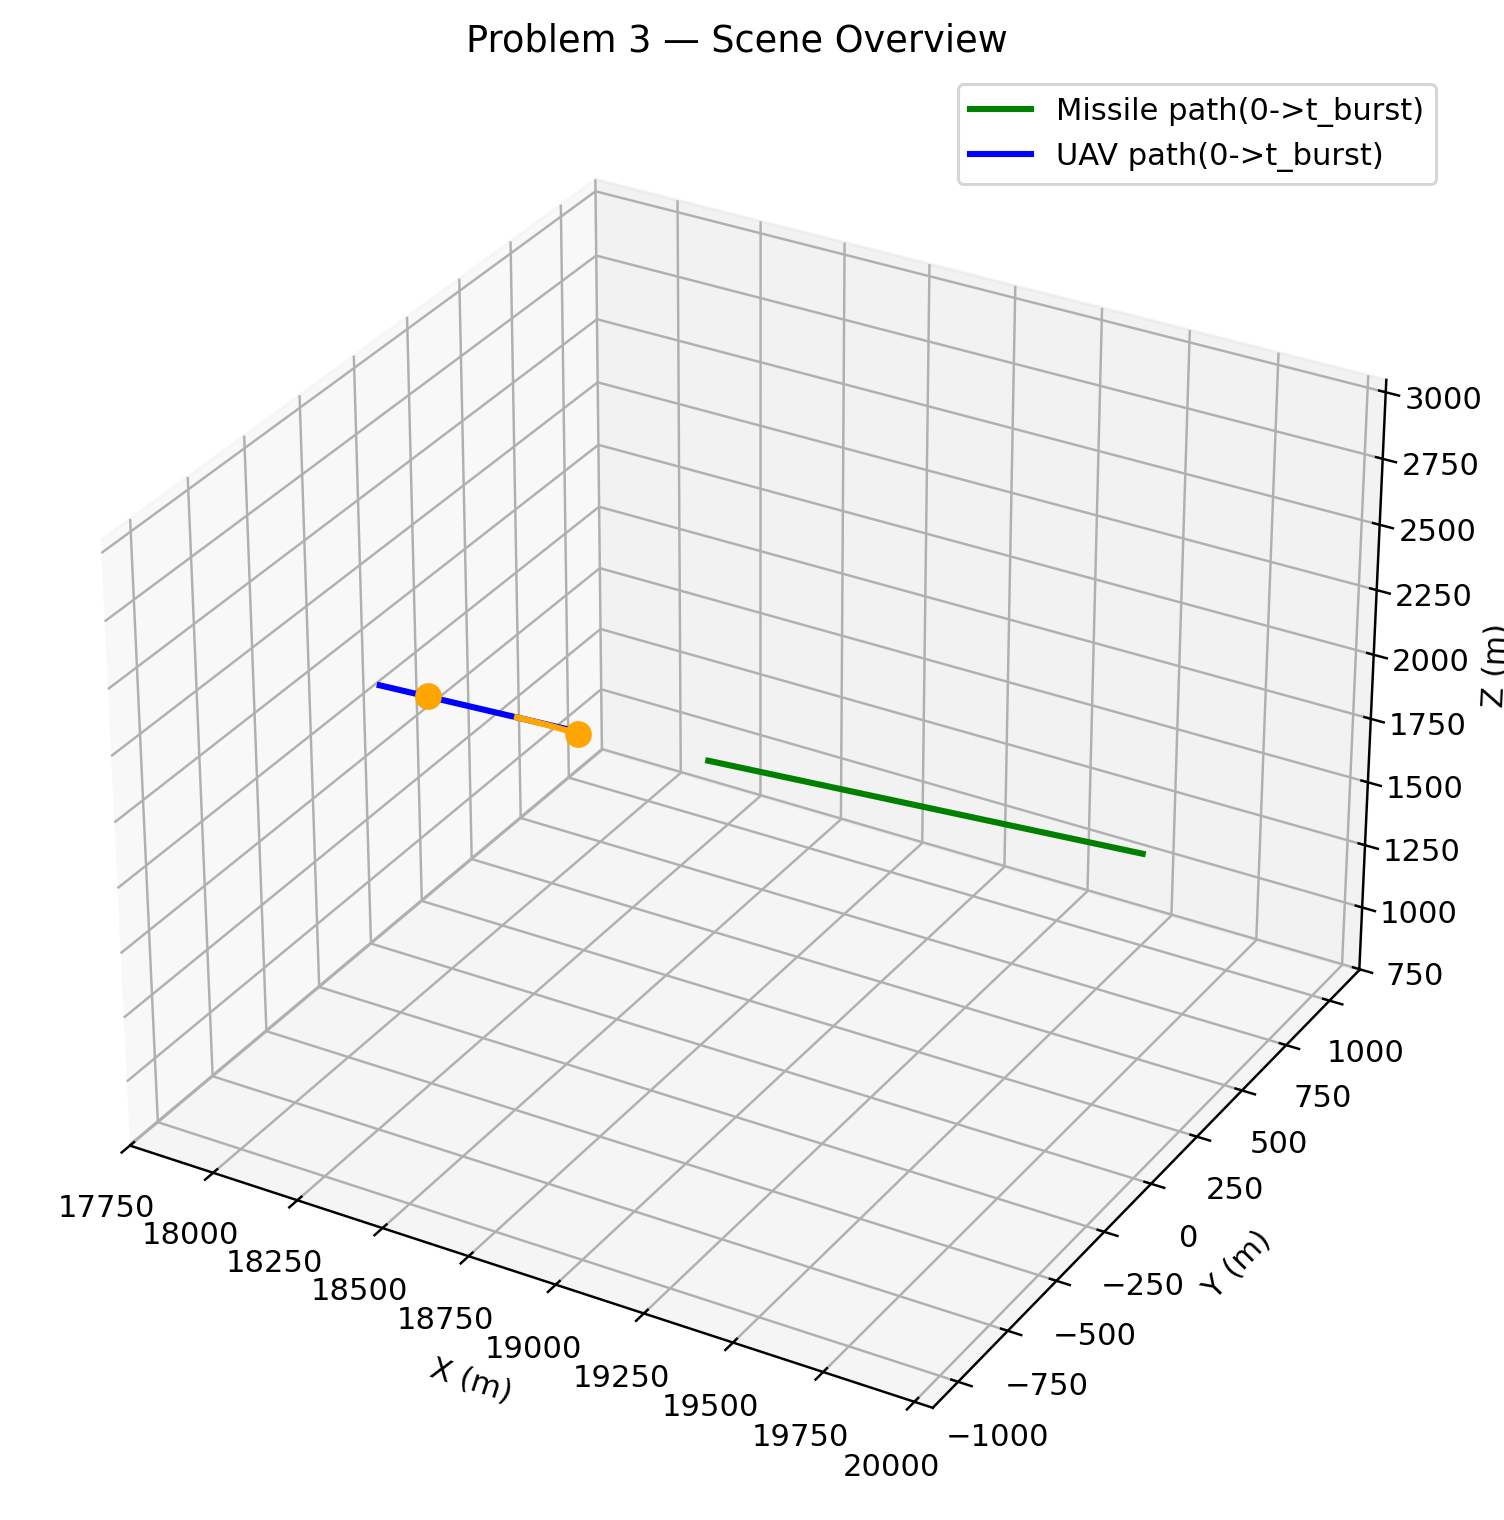
\includegraphics[width=.6\textwidth]{./figures/problem3_3d}
    \caption{问题3的三维场景图}
    \label{fig:problem3_3d}
\end{figure}

\begin{figure}[!h]
    \centering
    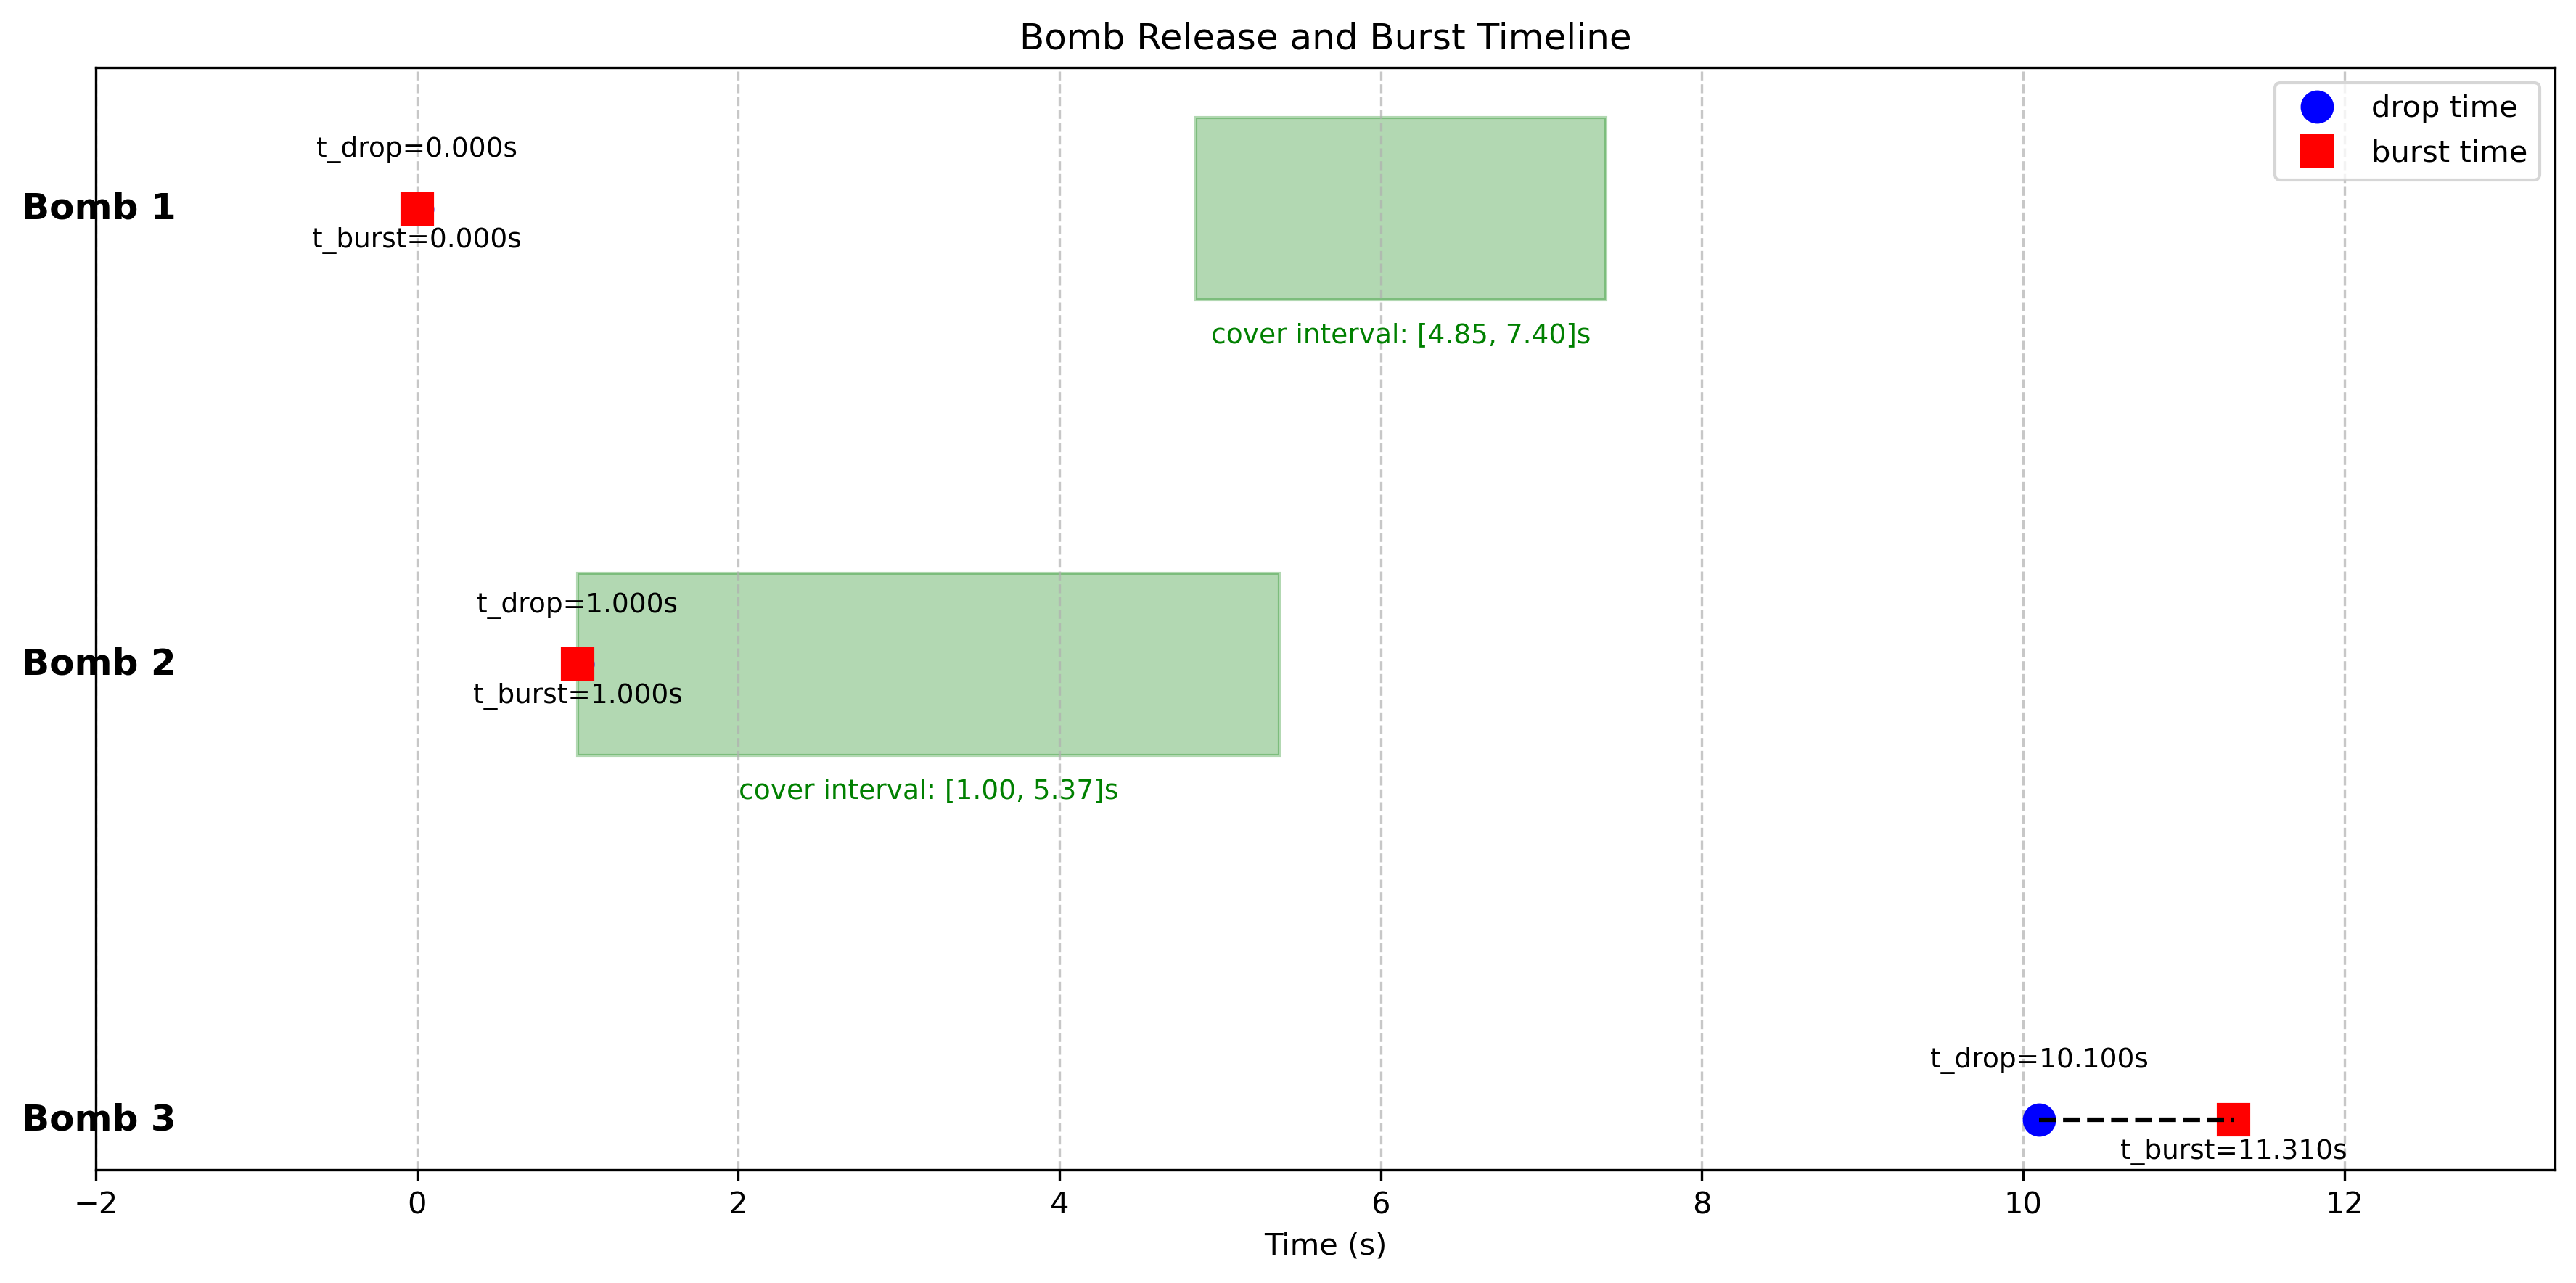
\includegraphics[width=\textwidth]{./figures/bomb_timeline_3}
    \caption{问题3投弹时间线}
    \label{fig:bomb_timeline_3}
\end{figure}

\subsection{问题四模型的建立与求解}

\subsubsection{模型的建立}
问题4是三架无人机各携带一枚烟幕干扰弹，目标是通过寻找合适的每架无人机的飞行速度，航向角，投弹时间，延时起爆时间，以期达到对单枚导弹M1遮蔽时间的最大化。本题采用三架无人机协同思路，先通过寻找每家无人机单独执行任务时最大化遮蔽时间的最优解，再通过检验遮蔽时间是否重叠，如若未重叠，那么三个局部最优解一定为全局最优解；如若重叠，再在此基础上去筛选其他更优解。

\textbf{单机决策与可行域}

对第 $i$ 架无人机，决策为
\[
x^{(i)}=\big(v_{\text{drone}}^{(i)},\ \theta^{(i)},\ t_{\text{drop}}^{(i)},\ \text{delay}^{(i)}\big),\qquad
t_{\text{burst}}^{(i)}=t_{\text{drop}}^{(i)}+\text{delay}^{(i)} .
\]

物理与边界约束逐行写为
\begin{align}
	v_{\min} &\le v_{\text{drone}}^{(i)} \le v_{\max},\\
	-\pi &\le \theta^{(i)} \le \pi,\\
	0 &\le t_{\text{drop}}^{(i)} \le T_{\text{end}},\\
	0 &\le \text{delay}^{(i)} \le T_{\text{effective}},\\
	t_{\text{burst}}^{(i)} &= t_{\text{drop}}^{(i)}+\text{delay}^{(i)} \ \le\ T_{\text{end}}.
\end{align}

若出现 $t_{\text{drop}}^{(i)}+\text{delay}^{(i)}>T_{\text{end}}$，在解码阶段作可行化修复：
\[
\text{delay}^{(i)}\leftarrow \max\!\big(0,\;T_{\text{end}}-t_{\text{drop}}^{(i)}\big),
\qquad
t_{\text{burst}}^{(i)}=t_{\text{drop}}^{(i)}+\text{delay}^{(i)} .
\]

\textbf{运动学与云团演化}

导弹从 $M_1^0$ 出发、以 $v_{\text{missile}}$ 指向 $\mathrm{fake}$ 匀速直线飞行：
\begin{equation}
	M_1^{t}
	= M_1^0
	+ v_{\text{missile}}\;t\;
	\frac{\mathrm{fake}-M_1^0}{\left\|\mathrm{fake}-M_1^0\right\|}.
\end{equation}

第 $i$ 架无人机等高匀速、航向角为 $\theta^{(i)}$。平抛可得其起爆位置
\begin{equation}
	P_{\text{burst}}^{(i)}
	=
	FY_i^0
	+ v_{\text{drone}}^{(i)}\,t_{\text{burst}}^{(i)}(\cos\theta^{(i)},\ \sin\theta^{(i)},\ 0)
	+ \big(0,\,0,\,-\tfrac12 g\,[\,t_{\text{burst}}^{(i)}-t_{\text{drop}}^{(i)}\,]^2\big).
\end{equation}

起爆后云团竖直下沉，评估时窗与云团中心为
\begin{gather}
	t\in\Big[t_{\text{burst}}^{(i)},\ \min\big(t_{\text{burst}}^{(i)}+T_{\text{effective}},\ T_{\text{end}}\big)\Big],\\
	C^{(i)}(t)=\Big(P_{\text{burst},x}^{(i)},\ P_{\text{burst},y}^{(i)},\ P_{\text{burst},z}^{(i)}-v_{\text{cloud}}\,[\,t-t_{\text{burst}}^{(i)}\,]\Big).
\end{gather}

\textbf{遮蔽判据与单机时长}

沿用问题一的“严格全覆盖”判据：对目标圆柱（底面中心 $real$、半径 $R$、高度 $H$）的可见表面均匀采样。若在某时刻 $t$ 对每个采样点 $B$ 都有
\begin{equation}
	\min_{s\in[0,1]}
	\left\|\,s\,M_1^{t}+(1-s)\,B - C^{(i)}(t)\,\right\|
	\ \le\ R_{\text{effective}},
\end{equation}

则认为该时刻被完全遮蔽。把满足条件的时刻并成区间集合 $\{[s_j^{(i)},e_j^{(i)}]\}$，定义单机有效遮蔽时长
\begin{equation}
	\text{CoverTime}^{(i)}=\sum_j \big(e_j^{(i)}-s_j^{(i)}\big).
\end{equation}

\paragraph{三机联合指标（并集）}
FY1 采用问题二的最优方案，FY2/FY3 为本题所得最优方案。三机遮蔽区间并集
\begin{equation}
	\mathcal{U}_{\text{all}}
	=\Big(\bigcup_j [s_j^{(1)},e_j^{(1)}]\Big)\ \cup\ \Big(\bigcup_j [s_j^{(2)},e_j^{(2)}]\Big)\ \cup\ \Big(\bigcup_j [s_j^{(3)},e_j^{(3)}]\Big).
\end{equation}
将 $\mathcal{U}_{\text{all}}$ 合并排序为若干不相交的区间 $[S_\ell,E_\ell]$，则
\begin{equation}
	\text{CoverTime}_{\text{all}}=\sum_{\ell}\big(E_\ell - S_\ell\big).
\end{equation}

\subsubsection{模型的求解}
先找到每架无人机单独执行任务时的最优解，再通过检验遮蔽时间是否重叠，如若未重叠，那么三个局部最优解一定为全局最优解；如若重叠，再在此基础上去筛选其他更优解。

\paragraph{单机优化（$i=1,2,3$ 独立求解）}
\begin{equation}
	\max_{\,v_{\text{drone}}^{(i)},\,\theta^{(i)},\,t_{\text{drop}}^{(i)},\,\text{delay}^{(i)}}
	\ \ \text{CoverTime}^{(i)}
	\quad
	\text{s.t. 上述边界与可行化约束。}
\end{equation}
实现采用实数编码的遗传算法：染色体
\[
[v_{\text{drone}}^{(i)},\ \theta^{(i)},\ t_{\text{drop}}^{(i)},\ \text{delay}^{(i)}],
\]

解码阶段计算 $t_{\text{burst}}^{(i)}$ 并执行可行化修复（保证 $t_{\text{burst}}^{(i)}\le T_{\text{end}}$）；适应度由严格判据下的区间集合 $\{[s_j^{(i)},e_j^{(i)}]\}$ 求得 $\text{CoverTime}^{(i)}$。为兼顾效率与精度，采用“粗评步长 + 精评步长”的两阶段评估：先用较大步长快速筛选，再对候选（含精英）以较小步长重评；进化操作为锦标赛选择、SBX 交叉与退火式高斯变异，并配以物理启发的初始种子以加速收敛。

\textbf{并集合并与结果导出}

得到 FY1–FY3 的最优区间后，按时间排序有序合并得到 $\mathcal{U}_{\text{all}}$ 与 $\text{CoverTime}_{\text{all}}$；同时导出每架无人机的
\[
(v_{\text{drone}}^{(i)},\ \theta^{(i)},\ t_{\text{drop}}^{(i)},\ \text{delay}^{(i)},\ t_{\text{burst}}^{(i)})
\]

及其投放/起爆三维坐标（与问题二相同的直线—平抛公式）用于展示与复现：
\begin{align}
	(x,y)_{\text{drop}}^{(i)} &= (FY_{i,x}^0, FY_{i,y}^0) + v_{\text{drone}}^{(i)}\,t_{\text{drop}}^{(i)}(\cos\theta^{(i)},\ \sin\theta^{(i)}),\\
	(x,y)_{\text{burst}}^{(i)}&= (FY_{i,x}^0, FY_{i,y}^0) + v_{\text{drone}}^{(i)}\,t_{\text{burst}}^{(i)}(\cos\theta^{(i)},\ \sin\theta^{(i)}),\\
	z_{\text{drop}}^{(i)}&=FY_{i,z}^0,\qquad
	z_{\text{burst}}^{(i)}=FY_{i,z}^0-\tfrac12 g\,[\,t_{\text{burst}}^{(i)}-t_{\text{drop}}^{(i)}\,]^2.
\end{align}

\begin{figure}
    \centering
    \begin{minipage}[c]{0.45\textwidth}
        \centering
        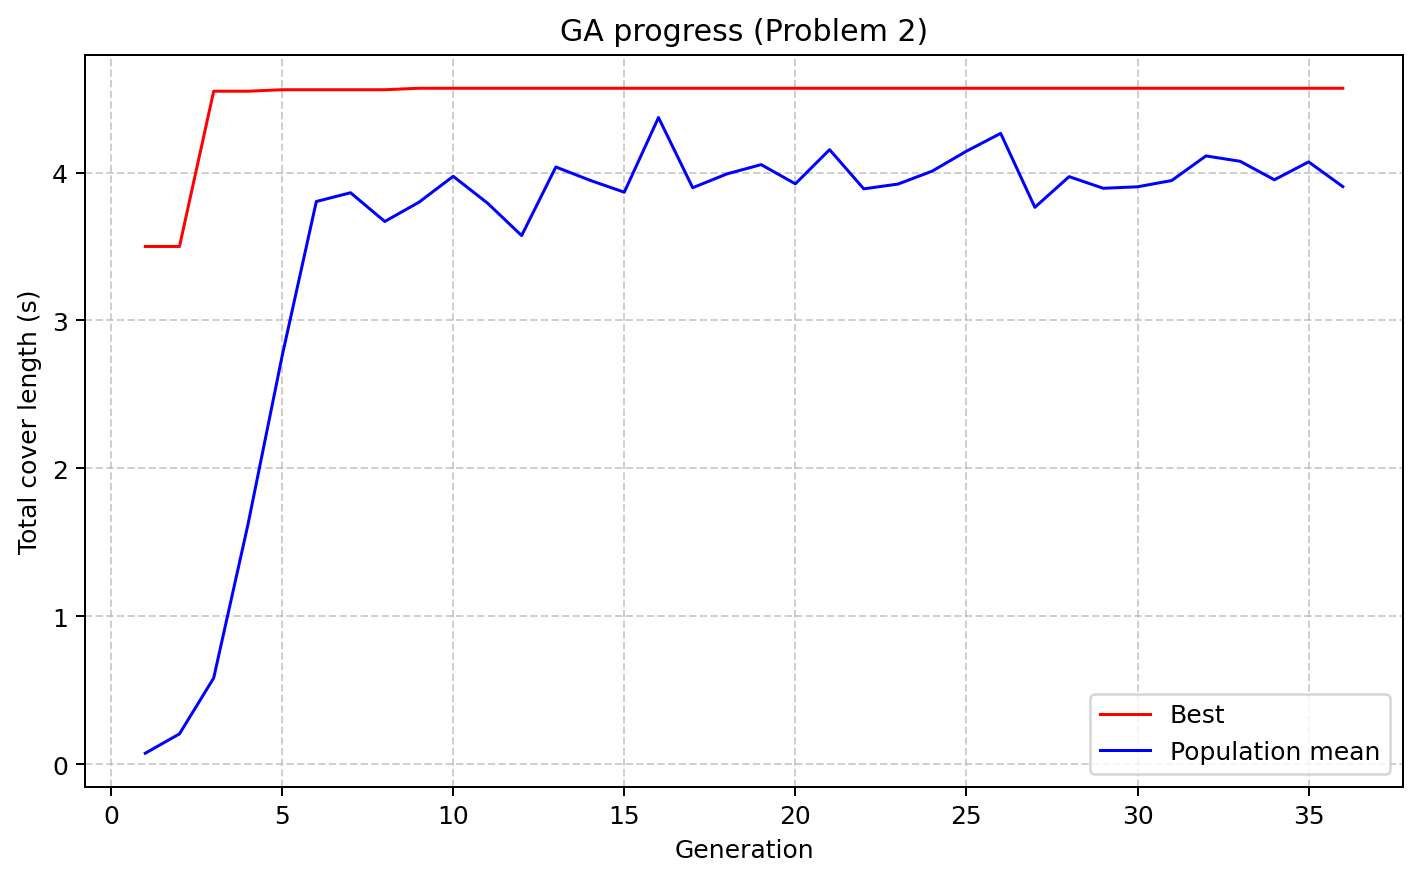
\includegraphics[width=0.95\textwidth]{./figures/problem2_ga_progress}
        \subcaption{FY1}
        \label{fig:fy1}
    \end{minipage}
    \begin{minipage}[c]{0.45\textwidth}
        \centering
        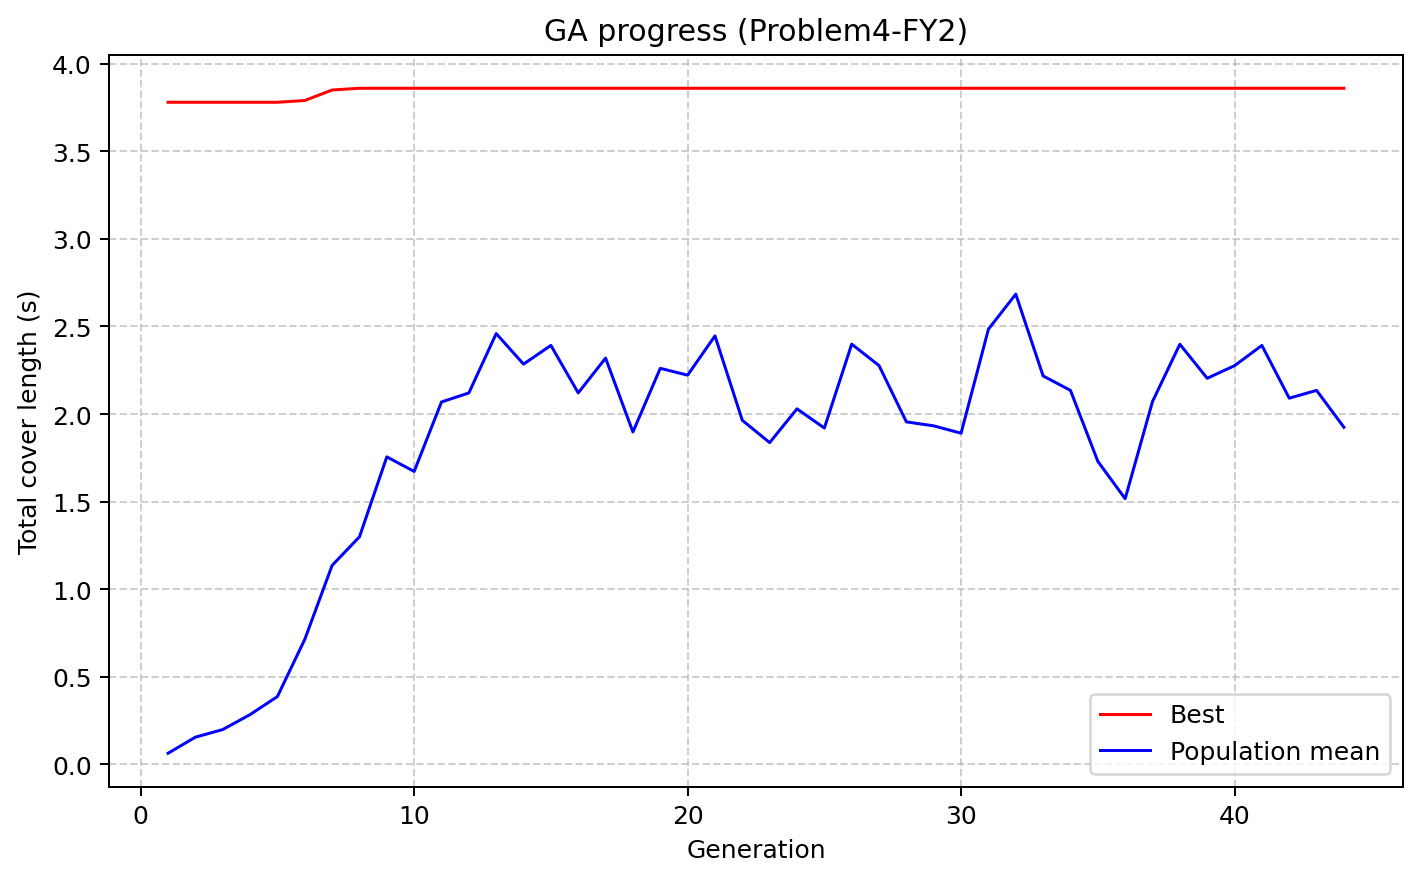
\includegraphics[width=0.95\textwidth]{./figures/fy2_ga_progress}
        \subcaption{FY2}
        \label{fig:fy2}
    \end{minipage}
    \begin{minipage}[c]{0.45\textwidth}
        \centering
        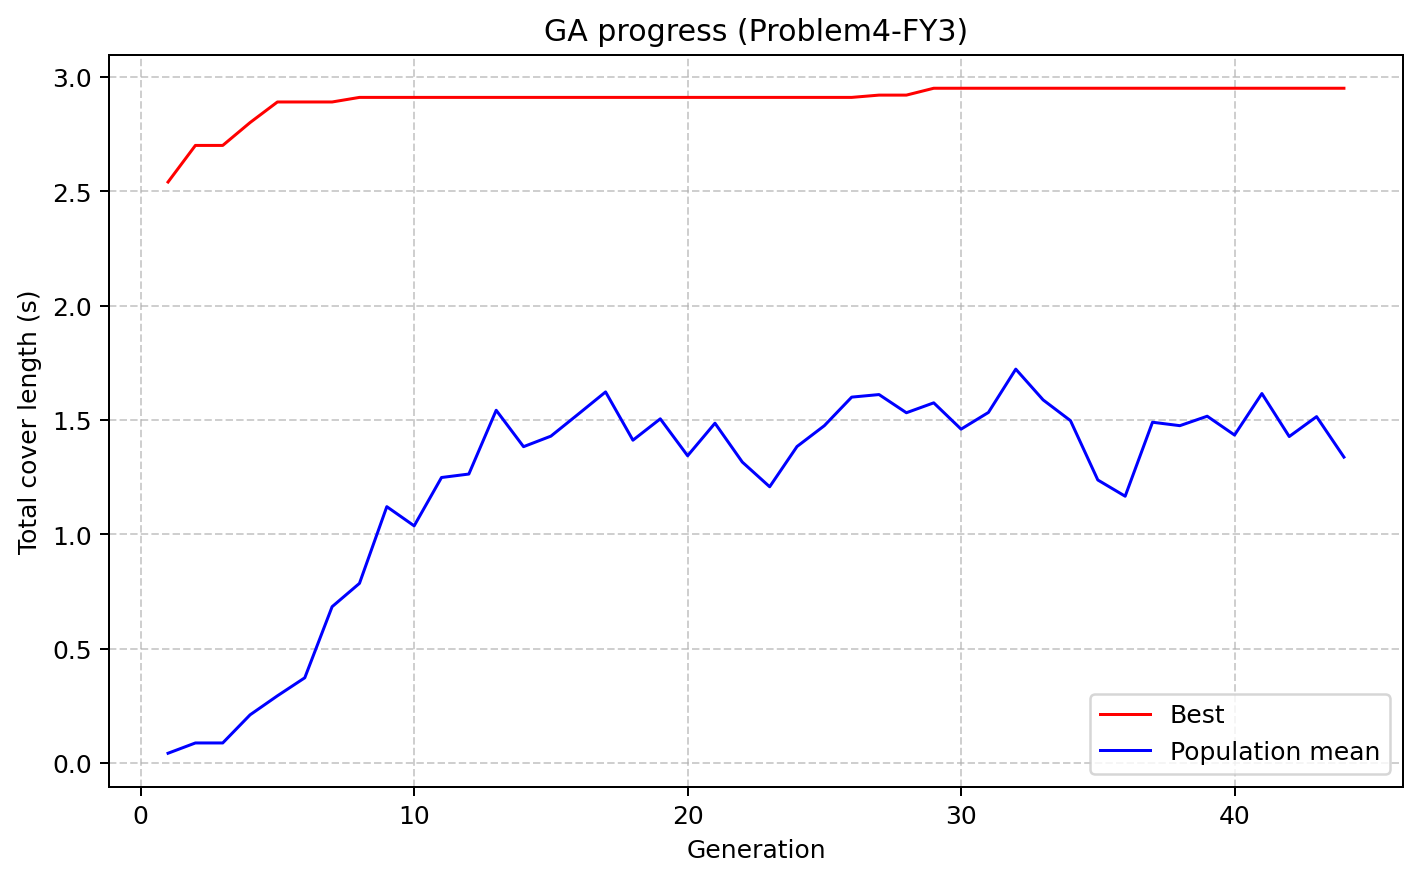
\includegraphics[width=0.95\textwidth]{./figures/fy3_ga_progress}
        \subcaption{FY3}
        \label{fig:fy3}
    \end{minipage}
    \caption{问题4遗传算法进展图}
    \label{fig:problem4_ga_progress}
\end{figure}

\textbf{最终结果为：}

最终对M1导弹的总有效遮蔽时间是 \textbf{11.38 s}。

\textbf{问题四总体参数}

\begin{table}[H]
	\centering
	\caption{炸弹参数数据}
	\label{tab:bomb_params}
	\begin{tabular}{l r r r r r r}
		\toprule
		\textbf{炸弹类型} & \textbf{覆盖长度(s)} & \textbf{速度(m/s)} & \textbf{航向(°)} & \textbf{投弹时间(s)} & \textbf{延迟(s)} & \textbf{爆炸时间(s)} \\
		\midrule
		FY1 & 4.570 & 74.623 & 6.371 & 0.461 & 0.793 & 1.254 \\
		FY2 & 3.860 & 140.000 & -44.883 & 11.067 & 2.980 & 14.047 \\
		FY3 & 2.950 & 110.016 & 89.460 & 23.833 & 4.268 & 28.101 \\
		\bottomrule
	\end{tabular}
\end{table}

\begin{figure}
    \centering
    \begin{minipage}[c]{0.45\textwidth}
        \centering
        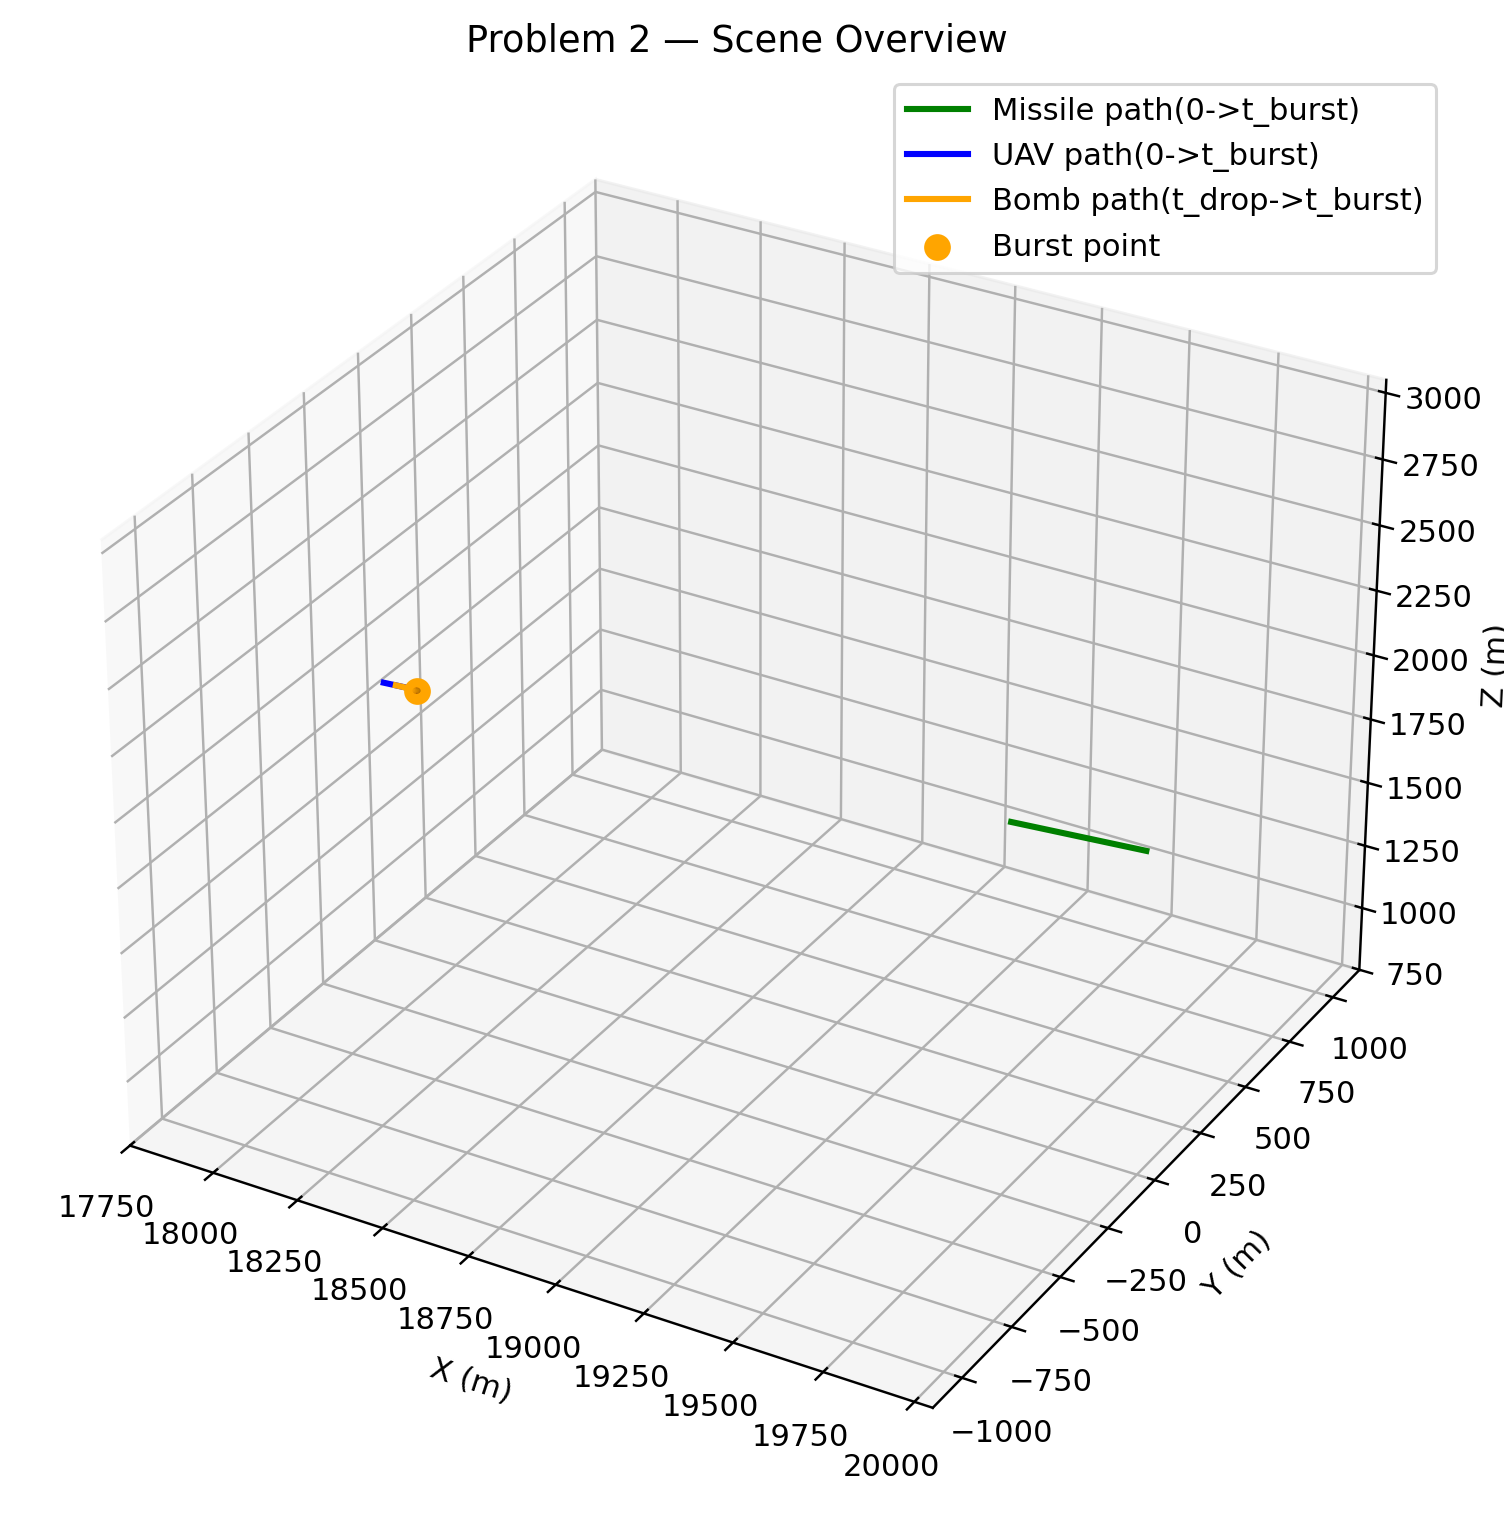
\includegraphics[width=0.95\textwidth]{./figures/problem2_3d}
        \subcaption{FY1}
        \label{fig:fy1}
    \end{minipage}
    \begin{minipage}[c]{0.45\textwidth}
        \centering
        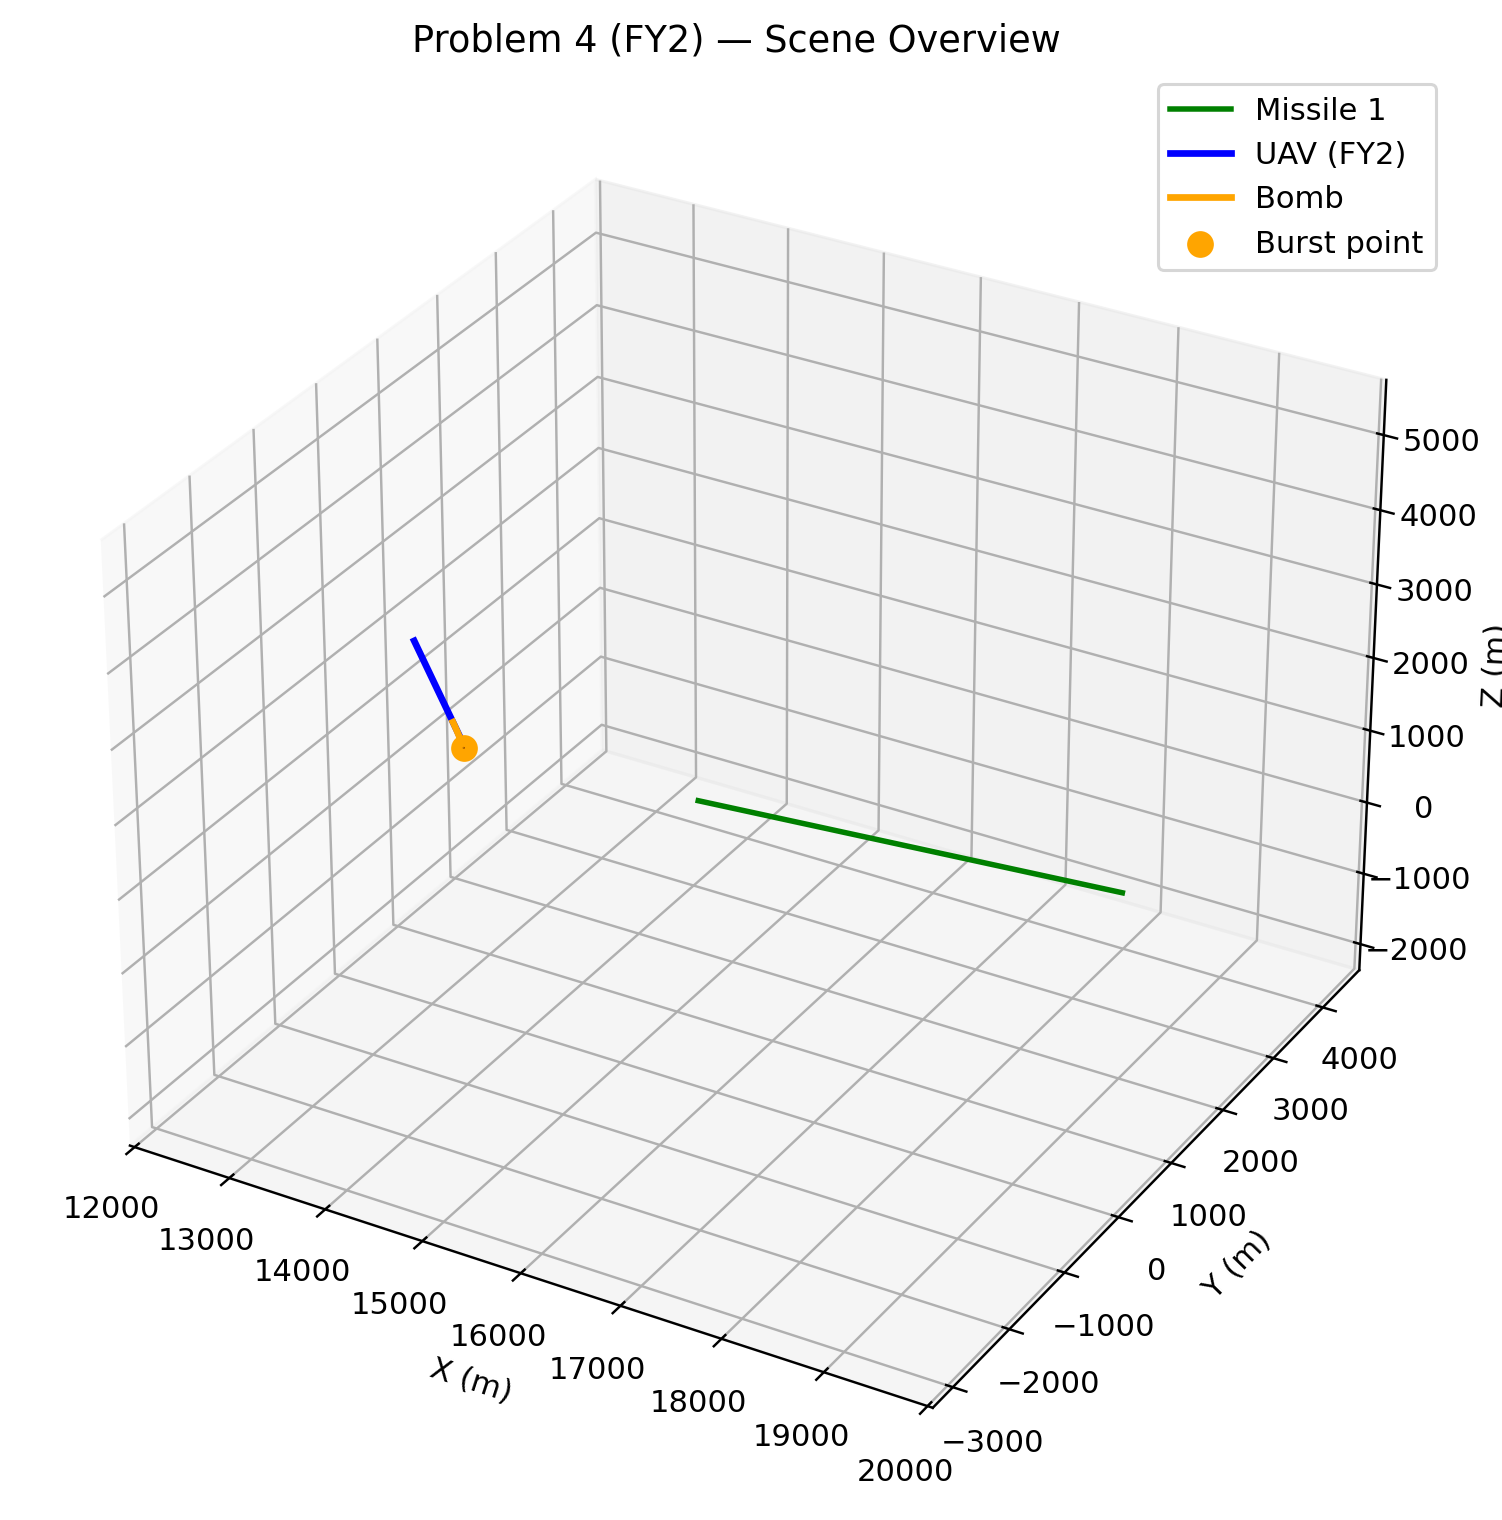
\includegraphics[width=0.95\textwidth]{./figures/problem4_fy2_3d}
        \subcaption{FY2}
        \label{fig:fy2}
    \end{minipage}
    \begin{minipage}[c]{0.45\textwidth}
        \centering
        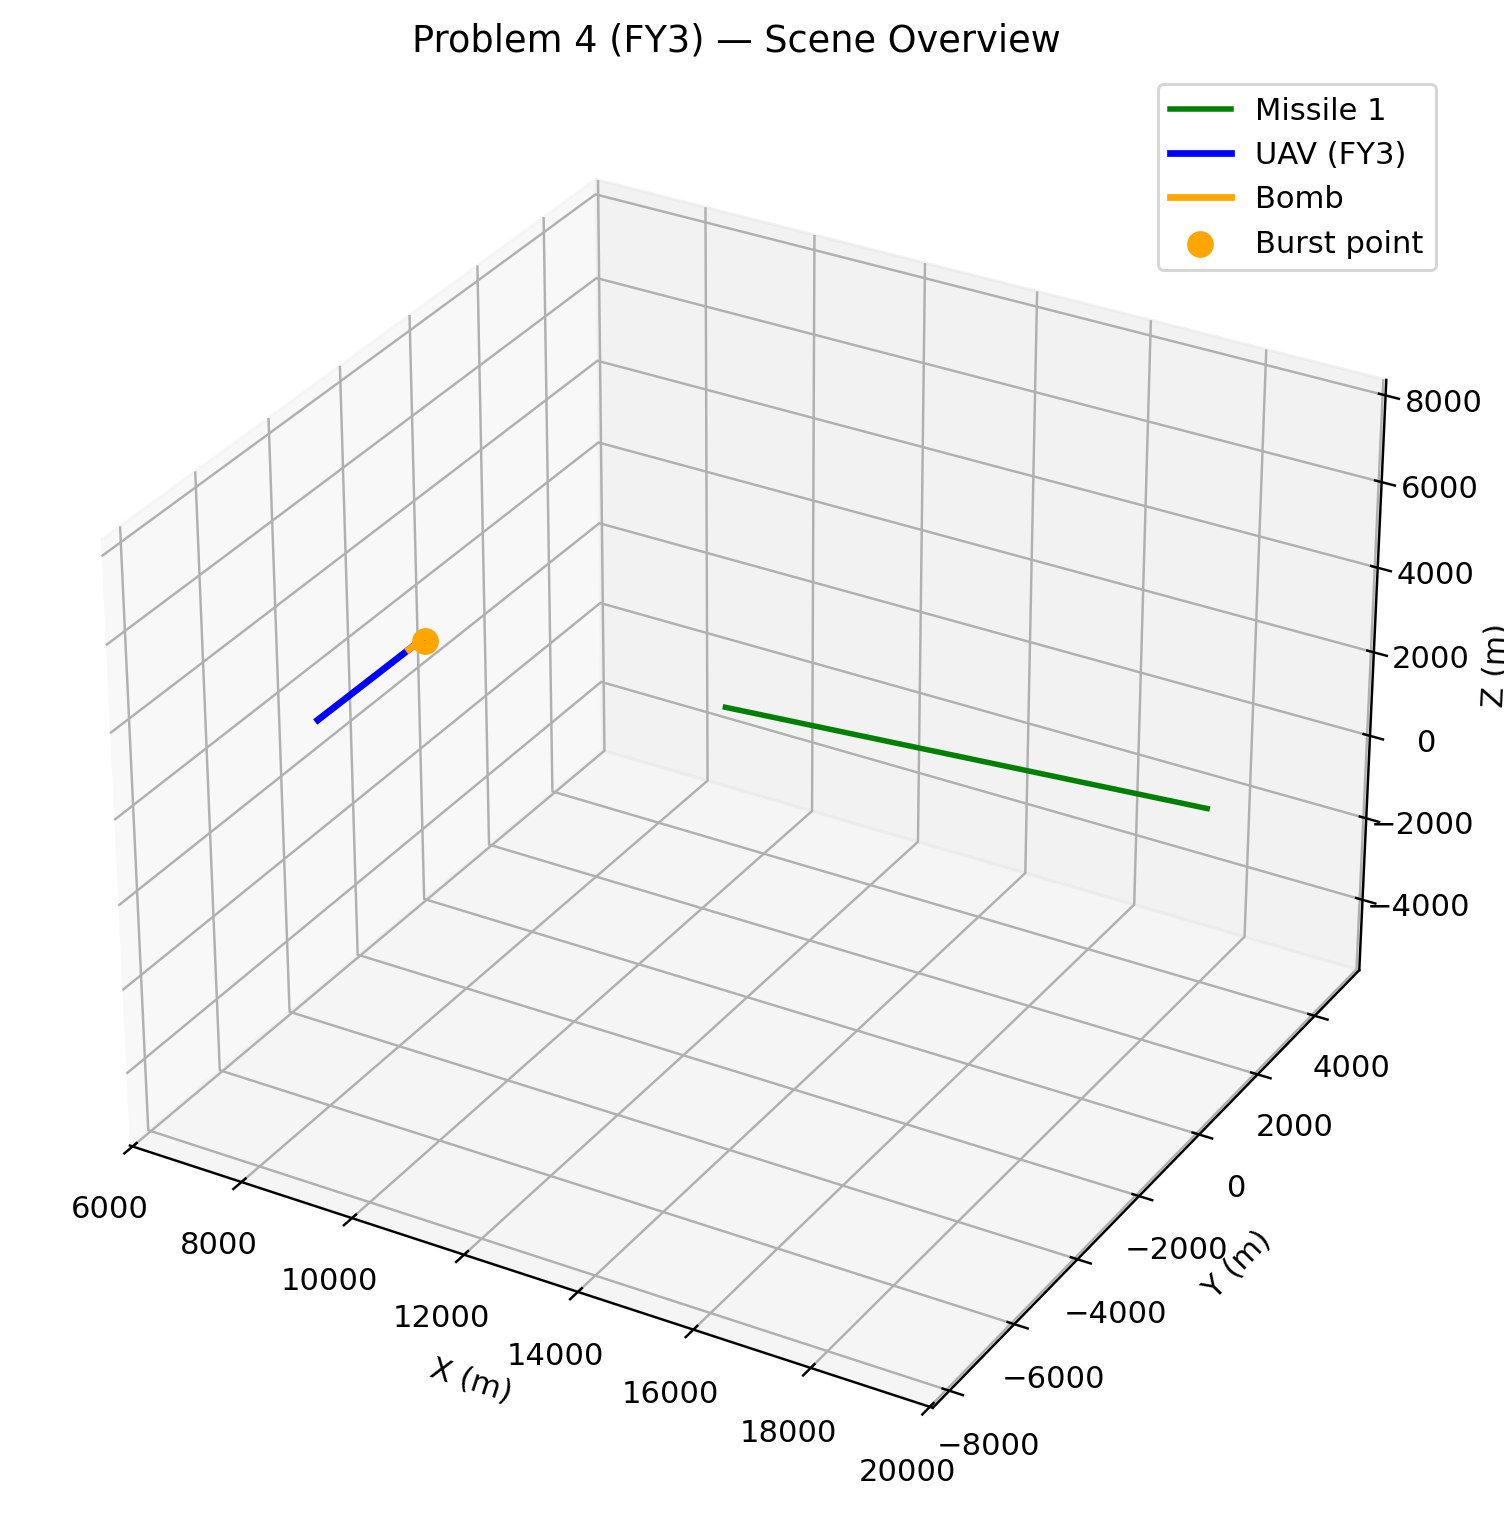
\includegraphics[width=0.95\textwidth]{./figures/problem4_fy3_3d}
        \subcaption{FY3}
        \label{fig:fy3}
    \end{minipage}
    \caption{问题4各无人机投弹轨迹}
    \label{fig:problem4_3d}
\end{figure}

\begin{figure}[!h]
    \centering
    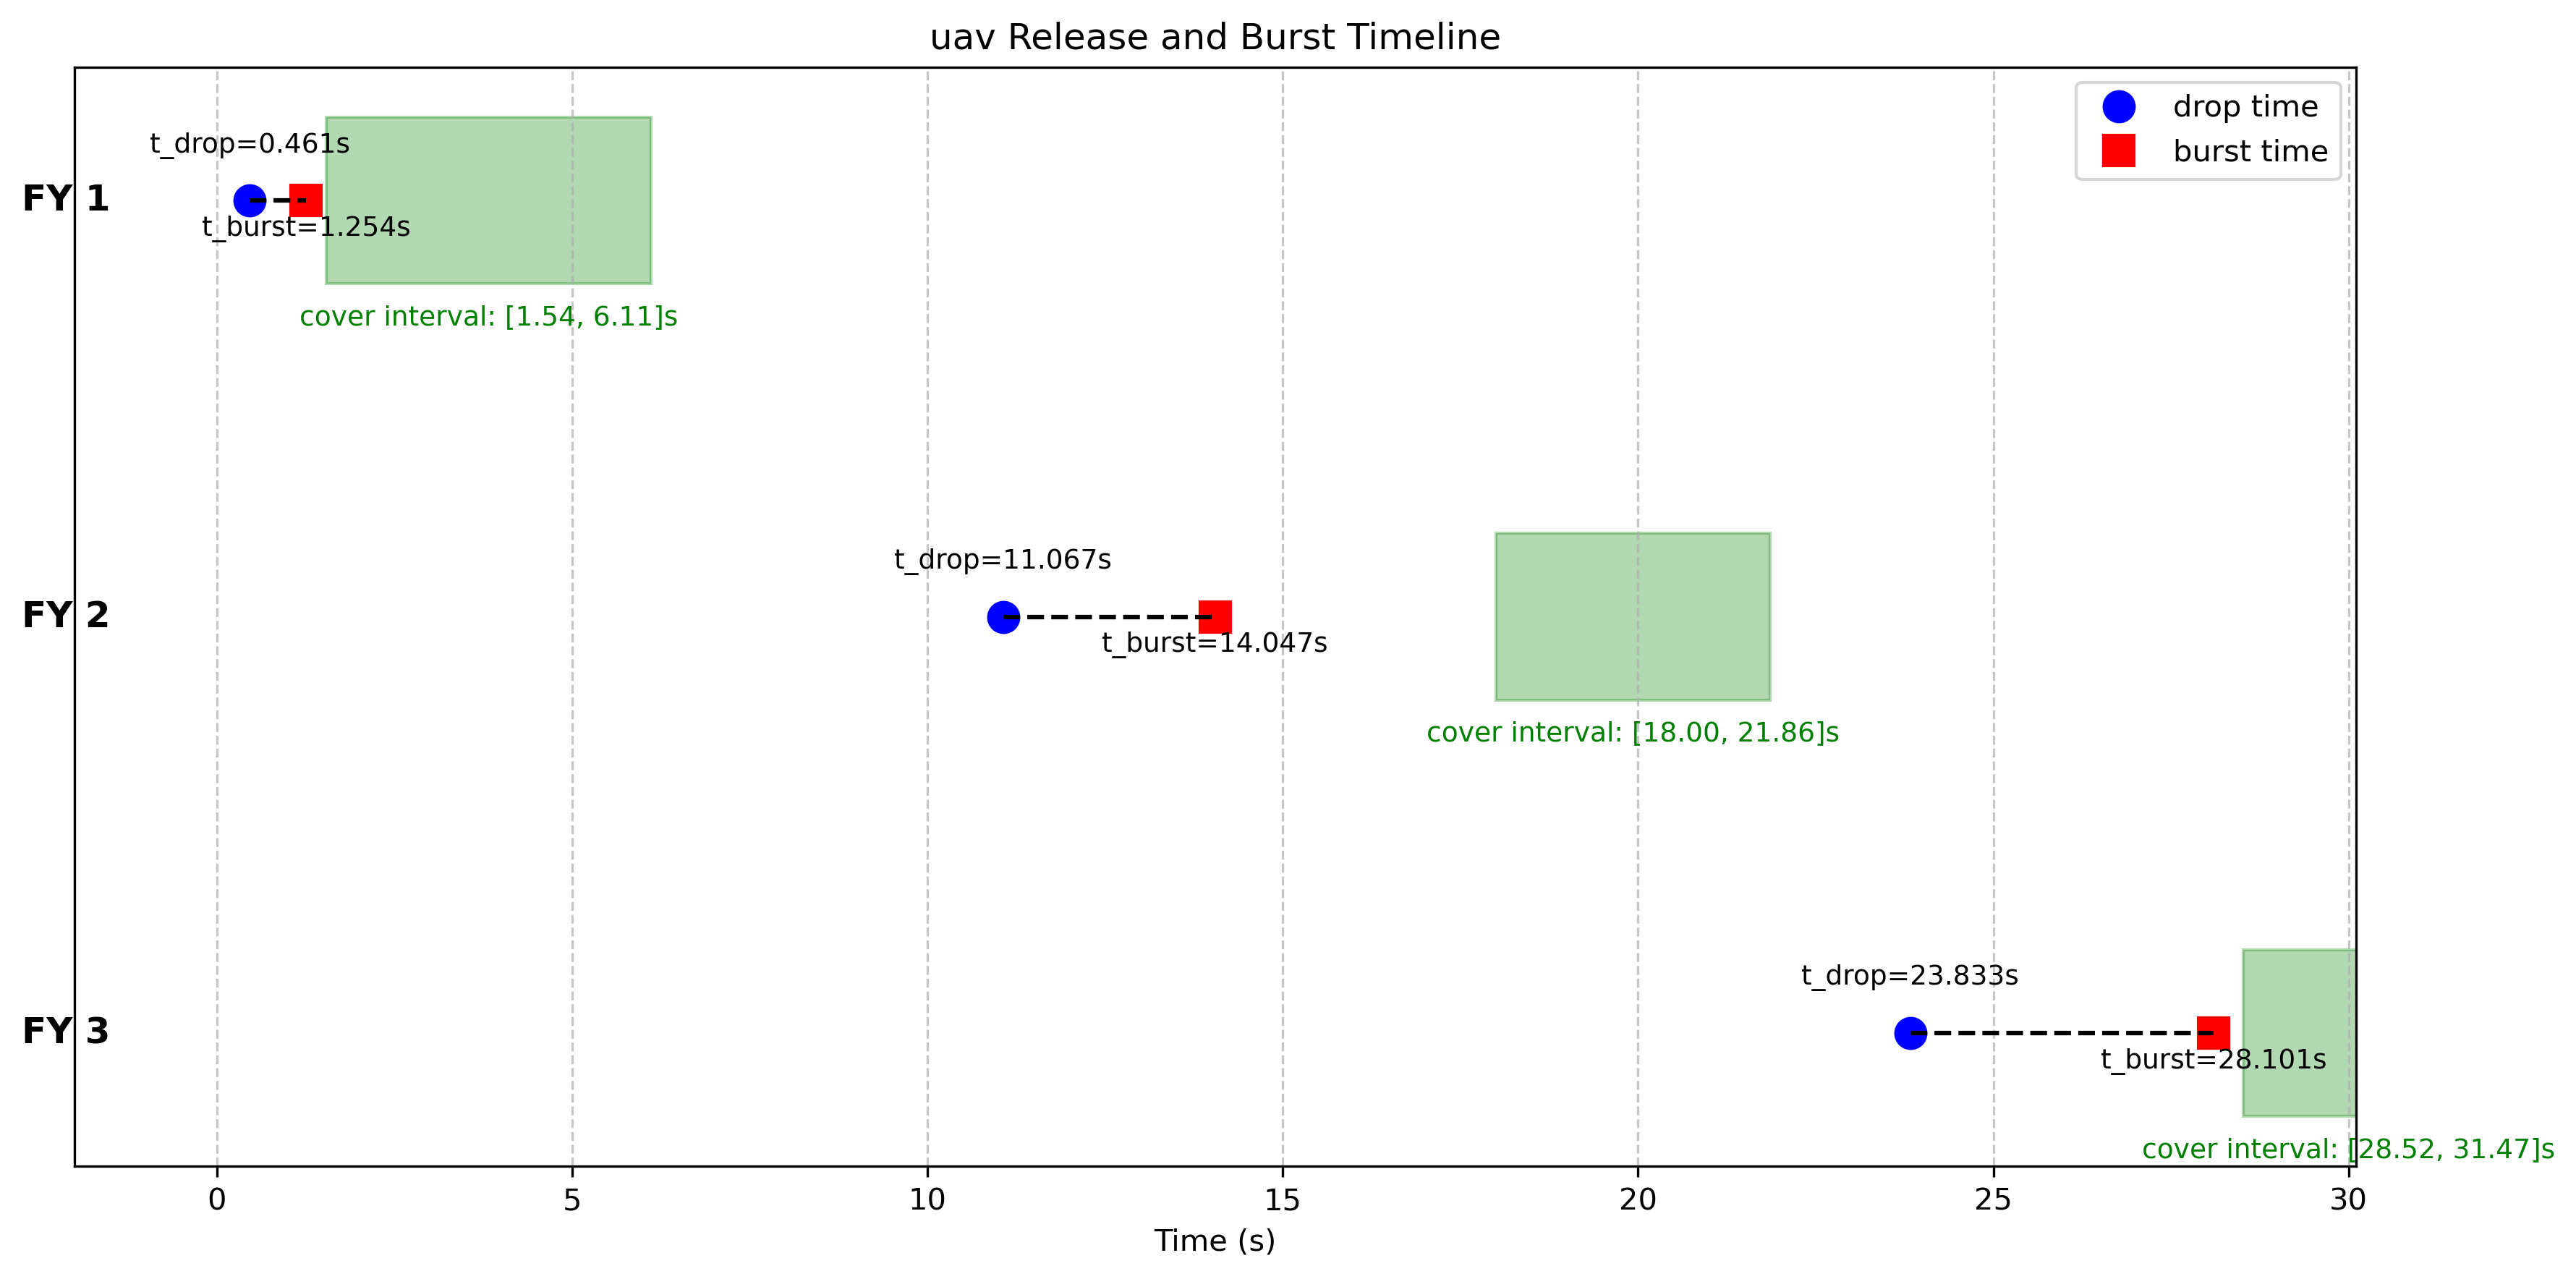
\includegraphics[width=\textwidth]{./figures/uav_timeline}
    \caption{问题4投弹时间线}
    \label{fig:uav_timeline}
\end{figure}

\subsection{问题五：模型的建立与求解}

\subsubsection{模型的建立}
本题是“多机×多弹×多导弹”的复杂题目，先从单架无人机的三次投放出发，定义运动学、评估时间窗与遮蔽判据；随后给出“按导弹分组取并集并求和”的计分方式，最后对五架无人机求和得到总目标。上标 $^{(i)}$ 表示第 $i$ 架无人机（$i=1,\dots,5$），上标 $^{(k)}$ 表示第 $k$ 次投放（$k=1,2,3$），导弹编号为 $m=1,2,3$。

\textbf{对象与时间轴}

三枚导弹均做等高匀速直线运动：
\begin{equation}
	M_m^{t}=M_m^{0}+v_{\text{missile}}\;t\;\frac{\mathrm{fake}-M_m^{0}}{\big\|\mathrm{fake}-M_m^{0}\big\|},\qquad m=1,2,3.
\end{equation}

第 $i$ 架无人机的决策量与起爆时刻：
\begin{equation}
	x^{(i)}=\Big(v_{\text{drone}}^{(i)},\ \theta^{(i)},\ \{t_{\text{rel}}^{(i,k)},\ \text{delay}^{(i,k)}\}_{k=1}^3\Big),\qquad
	t_{\text{burst}}^{(i,k)}=t_{\text{rel}}^{(i,k)}+\text{delay}^{(i,k)}.
\end{equation}

起爆点（平抛运动）：
\begin{equation}
	P_{\text{burst}}^{(i,k)}
	=FY_i^{0}
	+v_{\text{drone}}^{(i)}\,t_{\text{burst}}^{(i,k)}(\cos\theta^{(i)},\ \sin\theta^{(i)},\ 0)
	+\Big(0,\,0,\,-\tfrac12 g\,\big[t_{\text{burst}}^{(i,k)}-t_{\text{rel}}^{(i,k)}\big]^2\Big).
\end{equation}

云团中心与评估时间窗（为避免无效计算，引入统一上限 $T_{\cap}$）：
\begin{gather}
	C^{(i,k)}(t)=\Big(P_{x}^{(i,k)},\ P_{y}^{(i,k)},\ P_{z}^{(i,k)}-v_{\text{cloud}}\,[\,t-t_{\text{burst}}^{(i,k)}\,]\Big),\\
	t\in\Big[t_{\text{burst}}^{(i,k)},\ \min\big(t_{\text{burst}}^{(i,k)}+T_{\text{effective}},\ T_{\text{end}}\big)\Big]\cap[0,\,T_{\cap}],
\end{gather}
其中
\begin{equation}
	t_{\text{arr}}^{(m)}=\frac{\big\|\mathrm{fake}-M_m^{0}\big\|}{v_{\text{missile}}},\qquad
	T_{\cap}=\min\!\Big(T_{\text{end}},\ \max_{m\in\{1,2,3\}} t_{\text{arr}}^{(m)}\Big).
\end{equation}

\textbf{约束与可行化（与实现一致）}

\begin{align}
	v_{\min} &\le v_{\text{drone}}^{(i)}\le v_{\max},\\
	-\pi &\le \theta^{(i)}\le \pi,\\
	0 &\le t_{\text{rel}}^{(i,1)},\\
	t_{\text{rel}}^{(i,2)}-t_{\text{rel}}^{(i,1)} &\ge \text{interval},\\
	t_{\text{rel}}^{(i,3)}-t_{\text{rel}}^{(i,2)} &\ge \text{interval},\\
	0 &\le \text{delay}^{(i,k)}\le T_{\text{effective}},\quad k=1,2,3,\\
	t_{\text{burst}}^{(i,k)} &= t_{\text{rel}}^{(i,k)}+\text{delay}^{(i,k)}\ \le\ \min(T_{\text{end}},T_{\cap}).
\end{align}

为稳健起见，投放时刻采用差分编码并在解码时保证“严格间隔”：
\begin{equation}
	t_{\text{rel}}^{(i,1)}=d_1,\quad
	t_{\text{rel}}^{(i,2)}=t_{\text{rel}}^{(i,1)}+\text{interval}+d_2,\quad
	t_{\text{rel}}^{(i,3)}=t_{\text{rel}}^{(i,2)}+\text{interval}+d_3,\quad d_2,d_3\ge 0,
\end{equation}

若 $t_{\text{rel}}^{(i,k)}+\text{delay}^{(i,k)}$ 超出窗口上限，则在解码阶段对 $\text{delay}^{(i,k)}$ 做裁剪修复以满足可行性。

\textbf{遮蔽判据（严格全覆盖）与导弹分组并集}

对圆柱目标（底面中心 $real$、半径 $R$、高度 $H$）可见表面离散采样。若在时刻 $t$ 对\emph{每个}采样点 $B$ 均有
\begin{equation}
	\min_{s\in[0,1]}
	\Big\|\, s\,M_m^{t}+(1-s)\,B - C^{(i,k)}(t)\,\Big\|
	\ \le\ R_{\text{effective}},
\end{equation}

则判定“第 $i$ 架无人机的第 $k$ 次起爆在时刻 $t$ 对导弹 $m$ 形成完全遮蔽”，并将这些时刻并为若干区间。对固定 $(i,m)$，把三次起爆的区间取并集
\begin{equation}
	\mathcal{U}^{(i)}_{m}=\bigcup_{k=1}^{3}\ \bigcup_j [\,s_{j}^{(i,k,m)},\ e_{j}^{(i,k,m)}\,],
\end{equation}

其时长记为 $\operatorname{len}(\mathcal{U}^{(i)}_{m})$。单机目标定义为三枚导弹的并集时长之和
\begin{equation}
	\sum_{m=1}^{3}\operatorname{len}\!\big(\mathcal{U}^{(i)}_{m}\big),
\end{equation}

而总体目标为五架无人机之和
\begin{equation}
	\sum_{i=1}^{5}\sum_{m=1}^{3}\operatorname{len}\!\big(\mathcal{U}^{(i)}_{m}\big).
\end{equation}

\subsubsection{模型的求解}
求解策略沿用前文：把不可微、强几何约束的评估核固定在内层，外层以遗传算法（GA）在连续可行域上进行全局搜索；为控制代价且保证稳健，采用“粗评先筛、精评定分”的两阶段评估，并配合缓存与上界剪枝。

\textbf{五个单机子问题（互相独立）}
\begin{equation}
	\max_{\,v_{\text{drone}}^{(i)},\,\theta^{(i)},\,\{t_{\text{rel}}^{(i,k)},\text{delay}^{(i,k)}\}_{k=1}^{3}}
	\ \ \sum_{m=1}^{3}\operatorname{len}\!\big(\mathcal{U}^{(i)}_{m}\big)
	\quad \text{s.t. 上述边界与可行化约束},\quad i=1,\dots,5.
\end{equation}

实现细节：染色体
\[
[\ \theta^{(i)},\ v_{\text{drone}}^{(i)},\ d_1,\ \text{delay}^{(i,1)},\ d_2,\ \text{delay}^{(i,2)},\ d_3,\ \text{delay}^{(i,3)}\ ],
\]

解码生成 $t_{\text{rel}}^{(i,k)}$、$t_{\text{burst}}^{(i,k)}$ 并作可行化修复；粗评用较大步长并启用 \emph{快速充分判据} 预筛，精评用较小步长并以严格判据重评精英/候选；进化采用锦标赛选择、SBX 交叉与退火式高斯变异，并以物理可行的初始种子加速收敛。

\textbf{结果汇总与导出}

五个子问题最优后，直接求和得到总体目标；同时得到各无人机的最优参数
\[
(v_{\text{drone}}^{(i)},\,\theta^{(i)},\,t_{\text{rel}}^{(i,k)},\,\text{delay}^{(i,k)},\,t_{\text{burst}}^{(i,k)})
\]

及投放/起爆三维坐标（与前题相同的直线—平抛公式），并给出按导弹分组的区间并集时长明细，用于复现与对比。

\textbf{最终结果为：}

\textbf{问题五遮蔽时间汇总：}
\begin{table}[H]
	\centering
	\caption{问题五汇总}
	\label{tab:problem5_summary}
	\begin{tabular}{lc}
		\toprule
		指标 & 数值 \\
		\midrule
		FY1 总并集时长(s) & 6.4 \\
		FY2 总并集时长(s) & 5.28 \\
		FY3 总并集时长(s) & 5.41 \\
		FY4 总并集时长(s) & 0.0 \\
		FY5 总并集时长(s) & 5.18 \\
		总计(s) & 22.27 \\
		\bottomrule
	\end{tabular}
\end{table}

\begin{longtable}{p{0.14\textwidth}p{0.16\textwidth}p{0.14\textwidth}p{0.08\textwidth}p{0.22\textwidth}p{0.20\textwidth}}
	\caption{问题五结果}\label{tab:result5_details_2rows_long}\\
	\toprule
	\multicolumn{6}{l}{\textbf{第一行：姿态与时序}}\\
	无人机 & 航向角($^\circ$) & 速度(m/s) & 弹号 & 投放时刻 $t_{\text{rel}}$(s) & 延迟 $\tau$(s) \\
	\midrule
	\multicolumn{6}{l}{\textbf{第二行：坐标与指标}}\\
	\multicolumn{3}{l}{投放点坐标 (m)} & \multicolumn{2}{l}{起爆点坐标 (m)} & 有效时长(s) / 干扰导弹 \\
	\midrule
	\endfirsthead
	
	\toprule
	\multicolumn{6}{l}{\textbf{第一行：姿态与时序}（续）}\\
	无人机 & 航向角($^\circ$) & 速度(m/s) & 弹号 & 投放时刻 $t_{\text{rel}}$(s) & 延迟 $\tau$ (s) \\
	\midrule
	\multicolumn{6}{l}{\textbf{第二行：坐标与指标}}\\
	\multicolumn{3}{l}{投放点坐标 (m)} & \multicolumn{2}{l}{起爆点坐标 (m)} & 有效时长(s) / 干扰导弹 \\
	\midrule
	\endhead
	
	\midrule
	\multicolumn{6}{r}{Continued on next page}\\
	\midrule
	\endfoot
	
	\bottomrule
	\endlastfoot
	
	% === 数据区（每条两行）===
	FY1 & 5.012915 & 140.000000 & 1 & 0.000295 & 0.000000 \\
	\multicolumn{3}{l}{$(17800,\ 0,\ 1800)$} & \multicolumn{2}{l}{$(17800,\ 0,\ 1800)$} & $2.55\ /\ 1$ \\
	\addlinespace[2pt]
	
	FY1 & 5.012915 & 140.000000 & 2 & 1.001805 & 0.000000 \\
	\multicolumn{3}{l}{$(17937.12,\ 11.88975,\ 1800)$} & \multicolumn{2}{l}{$(17937.12,\ 11.88975,\ 1800)$} & $4.37\ /\ 1$ \\
	\addlinespace[2pt]
	
	FY1 & 5.012915 & 140.000000 & 3 & 10.097400 & 1.208209 \\
	\multicolumn{3}{l}{$(18192.04,\ 33.99482,\ 1800)$} & \multicolumn{2}{l}{$(18365.23,\ 49.01288,\ 1792.182)$} & $0.00\ /\ \textemdash$ \\
	\midrule
	
	FY2 & 295.073264 & 127.020000 & 1 & 7.910000 & 0.610000 \\
	\multicolumn{3}{l}{$(12424.5,\ 489.2,\ 1400)$} & \multicolumn{2}{l}{$(12457.1,\ 419.5,\ 1398.18)$} & $0.00\ /\ \textemdash$ \\
	\addlinespace[2pt]
	
	FY2 & 295.073264 & 127.020000 & 2 & 13.140000 & 2.680000 \\
	\multicolumn{3}{l}{$(12705,\ -112,\ 1400)$} & \multicolumn{2}{l}{$(12849,\ -421,\ 1364.81)$} & $3.81\ /\ 2$ \\
	\addlinespace[2pt]
	
	FY2 & 295.073264 & 127.020000 & 3 & 25.330000 & 6.500000 \\
	\multicolumn{3}{l}{$(13359,\ -1516,\ 1400)$} & \multicolumn{2}{l}{$(13708,\ -2263,\ 1192.98)$} & $1.47\ /\ 3$ \\
	\midrule
	
	FY3 & 91.394820 & 109.999400 & 1 & 23.774860 & 4.232581 \\
	\multicolumn{3}{l}{$(5937.5,\ -384,\ 700)$} & \multicolumn{2}{l}{$(5926.4,\ 80,\ 612.24)$} & $2.82\ /\ 1$ \\
	\addlinespace[2pt]
	
	FY3 & 91.394820 & 109.999400 & 2 & 27.194320 & 2.342137 \\
	\multicolumn{3}{l}{$(5928.5,\ -10,\ 700)$} & \multicolumn{2}{l}{$(5922.4,\ 250,\ 673.12)$} & $2.59\ /\ 2$ \\
	\addlinespace[2pt]
	
	FY3 & 91.394820 & 109.999400 & 3 & 28.356410 & 1.848465 \\
	\multicolumn{3}{l}{$(5925.5,\ 120,\ 700)$} & \multicolumn{2}{l}{$(5920.7,\ 320,\ 683.26)$} & $0.00\ /\ \textemdash$ \\
	\midrule
	
	FY4 & 0.000000 & 70.000000 & 1 & 0.920000 & 0.500000 \\
	\multicolumn{3}{l}{$(11064.4,\ 2000,\ 1800)$} & \multicolumn{2}{l}{$(11099.4,\ 2000,\ 1798.78)$} & $0.00\ /\ \textemdash$ \\
	\addlinespace[2pt]
	
	FY4 & 0.000000 & 70.000000 & 2 & 1.920001 & 1.340000 \\
	\multicolumn{3}{l}{$(11134.4,\ 2000,\ 1800)$} & \multicolumn{2}{l}{$(11228.2,\ 2000,\ 1791.2)$} & $0.00\ /\ \textemdash$ \\
	\addlinespace[2pt]
	
	FY4 & 0.000000 & 70.000000 & 3 & 2.920002 & 0.500000 \\
	\multicolumn{3}{l}{$(11204.4,\ 2000,\ 1800)$} & \multicolumn{2}{l}{$(11239.4,\ 2000,\ 1798.78)$} & $0.00\ /\ \textemdash$ \\
	\midrule
	
	FY5 & 120.108365 & 104.780075 & 1 & 15.962982 & 1.695641 \\
	\multicolumn{3}{l}{$(12161.5,\ -555,\ 1300)$} & \multicolumn{2}{l}{$(12072,\ -400,\ 1285.91)$} & $3.55\ /\ 1$ \\
	\addlinespace[2pt]
	
	FY5 & 120.108365 & 104.780075 & 2 & 17.493743 & 4.666900 \\
	\multicolumn{3}{l}{$(12080,\ -415,\ 1300)$} & \multicolumn{2}{l}{$(11835,\ 0,\ 1193.28)$} & $1.63\ /\ 2$ \\
	\addlinespace[2pt]
	
	FY5 & 120.108365 & 104.780075 & 3 & 23.308527 & 1.379184 \\
	\multicolumn{3}{l}{$(11775,\ 100,\ 1300)$} & \multicolumn{2}{l}{$(11705,\ 240,\ 1290.68)$} & $0.00\ /\ \textemdash$ \\
	% === 结束 ===
\end{longtable}


\section{模型的评价与推广}

\subsection{模型的评价}

\subsubsection{模型的优点}

\textbf{1} 模型并没有对真目标进行质点近似，且对有效遮蔽的判据进行了严格设计，相当精确地对投弹过程中的运动模型进行了数学描述，利用运动学公式和几何关系，能准确地在确定投弹策略的前提下计算出有效遮蔽时间。

\textbf{2} 求解时使用了遗传算法作为主要优化方法，这种算法可适应不同目标函数的初始条件，能准确地找到较优的投弹策略。

\textbf{3} 在问题四与问题五中采用了贪心算法进行优化，极大减少了直接求解的复杂度。

\subsubsection{模型的不足}

对复杂情景有较大的计算量，可能导致较高的计算时间，在现实中，缺乏反导系统需要的及时性。但是考虑军事用途，这些计算量对于军用级别的计算机来说是可以接受的。

\subsection{模型的推广}

基于遗传算法，问题五中的基因变量包含了五架无人机的航向、速度、三枚烟幕干扰弹的投放时间、引爆时间。过多的基因变量会使遗传算法的计算量陡增、计算时间过长和计算准确度下降，因此我们首先利用贪心算法将问题初步分解为五个独立的单机遮蔽三弹的优化子问题，再将结果汇总处理，不断迭代，使三枚导弹的有效遮蔽时间并集尽可能长


\begin{thebibliography}{99}
	
	\bibitem{Mezura2011CH}
	E. Mezura-Montes and C. A. Coello Coello,
	``Constraint-handling in nature-inspired numerical optimization: Past, present and future,''
	\textit{Swarm and Evolutionary Computation}, vol.~1, no.~4, pp.~173--194, 2011.
	
	\bibitem{Jiang2007}
	姜启源．\textit{数学模型}［M］．北京：高等教育出版社，2007年．
	
	\bibitem{Deb1995SBX}
	K. Deb and R. B. Agrawal,
	``Simulated Binary Crossover for Continuous Search Space,''
	\textit{Complex Systems}, vol.~9, no.~2, pp.~115--148, 1995.
	
	\bibitem{DeepSeek2025}
	DeepSeek-V3, DeepSeek-V3, 深度求索（DeepSeek），2025-09-07.
	
\end{thebibliography}

\newpage
%附录
\begin{appendices}

\section{支撑材料的文件列表}

\begin{itemize}
    \item code
    \begin{itemize}
        \item evaluator.py 评估模块
        \item funcs.py 通用函数
        \item ga.py 遗传算法模块
        \item params.py 参数文件
        \item problem1.py 问题一代码
        \item problem2.py 问题二代码
        \item problem3.py 问题三代码
        \item problem4\_fy2.py 问题四FY2代码
        \item problem4\_fy3.py 问题四FY3代码
        \item problem4.py 问题四代码
        \item problem5.py 问题五代码
        \item figure.py 绘图代码
        \item timeline1.py 问题一时间线
        \item timeline2.py 问题二时间线
        \item timeline3.py 问题三时间线
        \item timeline4.py 问题四时间线
    \end{itemize}
    
    \item result
    \begin{itemize}
        \item result1.xlsx 问题一结果
        \item result2.xlsx 问题二结果
        \item result3.xlsx 问题三结果
    \end{itemize}
    
    \item 数据结果.pdf
    
    \item AI工具使用详情.pdf
\end{itemize}

\section{源代码}

% 配置Python代码样式
\lstset{
  language=Python,       % 指定语言为Python
  basicstyle=\ttfamily\small,  % 基础字体
  keywordstyle=\color{blue},   % 关键字颜色
  commentstyle=\color{gray},   % 注释颜色
  stringstyle=\color{red},     % 字符串颜色
  numbers=left,          % 行号位置
  numberstyle=\tiny\color{gray},  % 行号样式
  frame=single,          % 边框样式
  showspaces=false,      % 不显示空格
  showstringspaces=false % 不显示字符串中的空格
}

以下是参数与通用函数代码：

\lstinputlisting{./code/evaluator.py}
\lstinputlisting{./code/funcs.py}
\lstinputlisting{./code/ga.py}
\lstinputlisting{./code/params.py}

以下是问题一的代码：

\lstinputlisting{./code/problem1.py}

以下是问题二的代码：

\lstinputlisting{./code/problem2.py}

以下是问题三的代码：

\lstinputlisting{./code/problem3.py}

以下是问题四的代码：

\lstinputlisting{./code/problem4_fy2.py}
\lstinputlisting{./code/problem4_fy3.py}
\lstinputlisting{./code/problem4.py}

以下是问题五的代码：

\lstinputlisting{./code/problem5.py}

以下是绘图代码：

\lstinputlisting{./code/figure.py}
\lstinputlisting{./code/timeline1.py}
\lstinputlisting{./code/timeline2.py}
\lstinputlisting{./code/timeline3.py}
\lstinputlisting{./code/timeline4.py}

\end{appendices}

\end{document}